\documentclass[preprint, 11pt]{elsarticle}
%\documentclass[final, 3p, 10pt]{elsarticle}

\usepackage[bitstream-charter]{mathdesign}      % nice font
\usepackage{amsmath}                            % lots of math typesetting
\usepackage{tikz}                               % pretty pictures
\usepackage{mathtools}                          % used for ceiling command
\usepackage{booktabs}                           % pretty tables
\usepackage{algorithm2e}                        % nice algorithms
\usepackage{imakeidx}                           % nice indexing
\usepackage{amsfonts}                           % special characters
\usepackage{listings}                           % to display code snippets
\usepackage{xspace}                             % helps spacing for \Detran
\usepackage[refpage]{nomencl}                   %
\usepackage{subcaption}
\usepackage{lscape}
\usepackage{threeparttable}
%\usepackage{fullpage}

\journal{Annals of Nuclear Energy}

\newcommand{\Detran}{{\tt Detran}\xspace}
\newcommand{\Serment}{{\tt Serment}\xspace}
\newcommand{\ie}{{\it i.e.}\xspace}
\newcommand{\eg}{{\it e.g.}\xspace}
\newcommand{\transp}{\mathsf{T}}
% Other helpful macros
\newcommand{\oper}[1]{\mathbf{#1}}

\begin{document}

\begin{frontmatter}

\title{Solving Eigenvalue Response Matrix Equations with 
       Nonlinear Techniques}

%% use optional labels to link authors explicitly to addresses:
%% \author[label1,label2]{<author name>}
%% \address[label1]{<address>}
%% \address[label2]{<address>}

\author[label1]{Jeremy A. Roberts\corref{cor1}}
\author[label2]{Benoit Forget}
\address[label1]{Department of Mechanical and Nuclear Engineering,
                 Kansas State University, 3002 Rathbone Hall, Manhattan, KS 66506, USA}
\address[label2]{Department of Nuclear Science and Engineering, 
                 Massachusetts Institute of Technology,
                 77 Massachusetts Avenue, 24-107, Cambridge, MA 02139, USA}
\cortext[cor1]{Corresponding author; email address: jaroberts@ksu.edu.}

\begin{abstract}
%% Text of abstract

This paper presents new algorithms for use in 
the eigenvalue response matrix method (ERMM) for reactor 
eigenvalue problems.  ERMM spatially decomposes a
 domain into independent nodes linked via
 boundary conditions approximated as 
truncated orthogonal expansions, the coefficients of which are  
response functions. 
In its simplest form, ERMM consists of a two-level 
eigenproblem: an outer Picard iteration updates the $k$-eigenvalue 
via balance,
while the inner $\lambda$-eigenproblem imposes neutron balance between nodes.  
Efficient methods are developed for solving the inner $\lambda$-eigenvalue 
problem within the outer Picard iteration. 
 Based on results from  
several diffusion and transport benchmark models, it was found that 
the Krylov-Schur method 
applied to the $\lambda$-eigenvalue problem reduces Picard solver 
times (excluding response generation) by a factor of 2--5. 
Furthermore, alternative methods including Picard acceleration schemes, Steffensen's 
method, and Newton's method are developed.  These approaches can 
yield faster $k$ convergence and a need for fewer
 $k$-dependent response function evaluations,
important because response computation is the 
largest cost for many problems.  It was found that
accelerating Picard iteration yields a reduction of 2--3 in total time 
compared to the unaccelerated case
for problems dominated by response generation but that 
Newton's method may provide nearly the same performance with improved 
robustness.
\end{abstract}

\begin{keyword}
%% keywords here, in the form: keyword \sep keyword

%% MSC codes here, in the form: \MSC code \sep code
%% or \MSC[2008] code \sep code (2000 is the default)
response matrix \sep reactor physics \sep neutron transport \sep eigenvalue
\end{keyword}

\end{frontmatter}

%-------------------------------*- Mode:TeX -*-------------------------------%
\section{Introduction and Background}
\label{sec:litreview}

Fundamental to reactor modeling is analysis of the steady-state 
balance of neutrons, described concisely as
\begin{equation}
  \oper{T} \phi(\vec{\rho}) = \frac{1}{k} \oper{F} \phi(\vec{\rho}) \, ,
  \label{eq:global}
\end{equation}
where the operator $\oper{T}$ describes transport processes, $\oper{F}$ 
describes neutron generation, $\phi$ is the neutron flux, $\vec{\rho}$ 
represents the relevant phase space, and $k$ is the eigenvalue, the ratio 
of the number of neutrons in successive generations. 

Since the late 1970's, full core analyses for light water reactors 
(LWR) have been performed using relatively low fidelity nodal methods 
based on clever homogenization of phase-space with proven success.  
However, as current reactors become increasingly heterogeneous 
due more aggressive fuel loadings and longer 
cycle lengths in existing LWR's, nodal methods are becoming less applicable, 
and for new, highly heterogeneous reactor designs, even less so. Although 
advances in production nodal codes, including use of generalized multigroup 
SP$_3$ transport with subassembly resolution, address issues related
to more complicated designs \cite{bahadir2009sng}, there likely is limited 
room for further improvement of the underlying approach.
Consequently, a move toward full core analysis techniques that can 
leverage the high fidelity methods typically used for smaller problems 
is desired.  


%============================================================================%
\subsection{The Eigenvalue Response Matrix Method}

One such approach is the response matrix method (RMM), which is 
based on a spatial decomposition of the global problem of Eq. \ref{eq:global}
into local fixed source problems connected by approximate boundary
conditions.
The response matrix method has been used in various forms since 
the early 1960's \cite{shimizu1963arm}.  Using the terminology of 
Lindahl and Weiss \cite{lindahl1981rrm}, the method can be formulated 
using explicit volume flux responses, called the ``source'' RMM, or by 
using current responses that include fission implicitly and hence are 
functions of $k$, known as the ``direct'' RMM.  Although both forms are 
used in various nodal methods, the source RMM is more widespread. 
This work is on the the direct RMM, which shall be referred to as the 
{\it eigenvalue} response matrix method (ERMM).

Several formulations of ERMM have been proposed since its first use in 
the 1960's. Here, a rather general approach is described based 
on expansions of the boundary conditions that couple
subvolumes of the global problem, a formalism introduced 
as early as the work of Lindahl \cite{lindahl1976mdr} and
studied more recently by several authors
\cite{mosher2006ifr, roberts2011ser, roberts2012ksi}.  

Suppose the global problem 
of Eq. \ref{eq:global} is defined over a 
volume $V$.  Then a local homogeneous problem can be defined over a 
subvolume $V_i$ subject to 
\begin{equation}
  \oper{T} \phi(\vec{\rho}_i) = 
    \frac{1}{k} \oper{F} \phi(\vec{\rho}_i) \, ,
  \label{eq:local}
\end{equation}
and
\begin{equation}
  J^{\mathrm{local}}_{-} (\vec{\rho}_{is}) = 
    J^{\mathrm{global}}_{-}(\vec{\rho}_{is}) \, ,
  \label{eq:localbc}
\end{equation}   
where $J^{\mathrm{local}}_{-} (\vec{\rho}_{is}) $ is a 
function of the incident boundary flux, typically the 
partial current, which quantifies net flows through a 
surface.

To represent the local problem numerically, an orthogonal basis, $P_n$,
over the relevant phase space is defined
\begin{equation}
  P_n(\vec{\rho}_{is}), \,\,\, n = 0, \, 1, \, \ldots N  \\
\end{equation}
subject to
\begin{equation}
   \int P_m(\vec{\rho}_{is}) P_n(\vec{\rho}_{is})  d\rho_{is}
     = \delta_{mn} \, .
\end{equation}
A response equation is defined 
\begin{equation}
 \oper{T} \phi_{i}^{ms} (\vec{\rho}_i) = 
   \frac{1}{k} \oper{F} \phi_{i}^{ms} (\vec{\rho}_i) 
\end{equation}
subject to
\begin{equation}
 J^{\mathrm{local}}_{-} (\vec{\rho}_{is}) = P_m(\vec{\rho}_{is}) \, .
\end{equation}
The resulting outgoing currents $J_{-} (\vec{\rho}_{is}) $ are used to define
response functions
\begin{equation}
       r^{ms}_{im's'} = \int  P_{m'}(\vec{\rho}_{is'})  
        J_{i+}^{m} (\vec{\rho}_{is'}) d\rho_{is'} \, .
\label{eq:responsefunction}
\end{equation}
The quantity $r^{ms}_{im's'}$ has a simple physical
interpretation: it is the $m'$th order response 
out of surface $s'$ due to a unit incident $m$th order condition on 
surface $s$ of subvolume $i$. 

The incident and outgoing currents are expressed as
truncated expansions using the same basis
\begin{equation}
  J_{is\pm}(\vec{\rho}_{is}) \approx \sum^{N}_{n=0}  
    j^n_{is_\pm} P_n (\vec{\rho}_{is}) 
\end{equation}
where
\begin{equation}
      j^n_{is_\pm} = \int  P_n (\vec{\rho}_{is}) 
        J_{\pm} (\rho_{is}) d \rho_{is} \, .
\end{equation}
These coefficients are then represented in vector form as
\begin{equation}
  \mathbf{J}_{i\pm} = ( j^0_{i1_\pm} \, j^1_{i1_\pm} \, \ldots \, 
    j^0_{i2_\pm} \, j^1_{i2_\pm} \, \ldots \, j^N_{iS_\pm} )^\mathsf{T} \, ,
\end{equation}
and using these together with Eq. \ref{eq:responsefunction} yields
the nodal balance equation
\begin{equation}
    \mathbf{J}_{i+} = 
%     \left [\begin{array}{c}
%       j^0_{i1_+}    \\
%       j^1_{i1_+}    \\
%       \vdots        \\
%     \end{array} 
%     \right ] =
     \left [\begin{array}{ccc}
       r^{01}_{i01} &  r^{11}_{i01}  &  \cdots   \\
       r^{01}_{i11} &  r^{11}_{i11}  &  \cdots   \\
                    &                &  \ddots   \\
    \end{array} 
    \right ] \left [\begin{array}{c}
      j^0_{i1_-}       \\
      j^1_{i1_-}       \\
      \vdots           \\
    \end{array} 
    \right ] = \mathbf{R}_i\mathbf{J}_{i-} \, .
  \label{eq:elementresponse}
\end{equation}

Global balance is defined by the eigenvalue response matrix
equation
\begin{equation}
  \oper{M}\mathbf{R}(k)\mathbf{J_-}  = \lambda \mathbf{J_-} \, ,
  \label{eq:erme}
\end{equation}
where 
$\oper{R}$ is the block diagonal response matrix of $\oper{R}_i$,  
$\mathbf{J}_{-}$ are vectors containing all incident current coefficients, 
$\oper{M}=\oper{M}^\mathsf{T}$ is 
the connectivity matrix that redirects outgoing responses as incident
responses of neighbors, superscript $\mathsf{T}$ represents the matrix 
transpose, and $\lambda$ is an eigenvalue that
represents the global balance of neutron currents through all 
nodal surfaces.
If the response matrix $\oper{R}$ is conservative (i.e. it
strictly maintains neutron balance),
\begin{equation}
 \lim_{k\to k^*} \lambda = 1 \, ,
\end{equation}
where $k^*$ is the true eigenvalue.
For nonconservative response expansions, the deviation of $\lambda$ from
unity measures discontinuities introduced across node boundaries and 
may be used to evaluate accuracy of the expansions used (with 
respect to an infinite expansion).


The $k$-eigenvalue can be interpreted physically as the ratio of neutrons
produced in one generation to the previous generation. 
Alternatively, $k$ can be viewed as the ratio of gains to losses in a given 
generation, and when applying this interpretation to the response matrix 
formalism, $k$ can be updated via the process
\begin{equation}
  k_{n+1} = \frac{\mathbf{F}(k_{n})\mathbf{J}_{-}} 
  { \mathbf{A}(k_{n}) \mathbf{J}_{-} + \mathbf{L}(k_{n}) \mathbf{J}_{-} }\, ,
\label{eq:picard}
\end{equation}
where $\oper{F}(k)\mathbf{J}_{-}$ is the global fission rate, 
$\oper{A}(k) \mathbf{J}_{-}$ is the global absorption rate,
and $\oper{L}(k) \mathbf{J}_{-}$ is the total leakage rate
from global boundaries.

%===========================================================================%
\subsection{Survey of ERMM Implementations}

The method defined by Eqs. \ref{eq:local}-\ref{eq:picard}
originates from the work of Shimizu et al. 
\cite{shimizu1963rmm, shimizu1963arm}, which appears to be the first work 
on response matrix methods (although the authors acknowledged a 
connection between their work and the earlier and more general 
theory of invariant imbedding as developed by Bellman et al. 
\cite{bellman1960iim}).  The method was originally based on 1-D diffusion 
in slab geometry. Aoki and Shimizu extended the approach to two dimensions, 
using a linear approximation in space to represent boundary
currents \cite{aoki1965arm}.
A shortcoming of this early work was an assumed value (unity) of 
the $k$-eigenvalue when evaluating responses, following which 
Eqs. \ref{eq:erme} and \ref{eq:picard} were solved just once 
to compute $k$.
Typically $k \approx 1$ for nuclear reactors, so the errors observed 
were only tens of pcm, which may have been deceptively small
and not representative of more general cases.  
In the later 2-D analysis \cite{aoki1965arm}, the results compared 
favorably to fine mesh diffusion calculations.

Weiss and Lindahl generalized ERMM by considering arbitrarily 
high order expansions of the boundary currents in Legendre 
polynomials \cite{weiss1975hor} and introducing an 
iterative sceheme for the $k$-eigenvalue equivalent to Eq. \ref{eq:picard}.
Lindahl also studied expansions of the current, comparing Legendre 
expansions to an approach that divides the boundary in several segments 
in which the current is assumed flat \cite{lindahl1976mdr}.  A more
complete overview of these approaches can be found in the review by Lindahl
and Weiss \cite{lindahl1981rrm}.

These diffusion-based methods rely on semi-analytic solutions to the 
diffusion equation and hence require homogeneous nodes. Previous 
scoping studies examined diffusion-based responses using discretized 
operators \cite{roberts2011ser}.  By numerically integrating the diffusion 
equation, heterogeneous nodes are treated naturally, though no diffusion 
models with heterogeneous nodes were studied.


In addition to methods based on diffusion theory, previous work applied 
transport theory for generating responses. Pryor et al. used 
a hybrid stochastic-deterministic approach based on
Monte Carlo and the collision probability 
method to generate responses \cite{pryor1973rmm, pryor1975rdr,
sicilian1975atr}.  Their work is unique in its definition
of the response matrix $\oper{R}(k)$ based on a precomputed 
series expansion.  Considering again Eq. \ref{eq:local}, the 
solution $\phi$ (omitting 
indices) can
be expressed as
\begin{equation}
 \phi = \phi_{0} + \frac{1}{k}\phi_{1}
                 + \frac{1}{k^2}\phi_{2}  + \ldots \, ,
\end{equation}
where $\phi_{i} $ is the flux for the $i$th neutron
generation due to fission.  The 
associated responses can be similarly defined
\begin{equation}
 \oper{R}(k) = \oper{R}_0 + \frac{1}{k}\oper{R}_1
                 + \frac{1}{k^2}\oper{R}_2  + \ldots \, .
\label{eq:responsesum}
\end{equation}
The authors claim this series can be truncated in as few as three terms 
by estimating the analytical sum, though the accuracy is not 
specified \cite{sicilian1975atr}.  When no fissile material is present, 
$\phi_{i} = 0$ for $i > 0$, and so $\oper{R}(k) = \oper{R}_0$.


A somewhat similar approach was developed by 
Moriwaki et al. \cite{moriwaki1999ndc}
in which Monte Carlo is used to 
generate assembly-level responses for full core analyses. 
Their method decomposes the response
matrix into four physically distinct components: 
transmission of incident neutrons from one surface to another surface ($T$), 
escape of neutrons born in the volume out of a surface ($L$), 
production of neutrons in the volume due to neutrons born in the 
volume ($A$), and production of neutrons in the volume due to neutrons 
entering a surface ($S$). If all indices but the 
surface are neglected, a current response can be expressed as
\begin{equation}
 r^{s}_{t} = T^s_t + \frac{1}{k}S^s(L_t + \frac{1}{k}A(L_t 
                   + \frac{1}{k}A(L_t + \cdots )) + \cdots) \, .
\label{eq:responseiterate}
\end{equation}
Like Eq. \ref{eq:responsesum}, this infinite sum 
represents the contributions of each generation to the 
total response.  The
matrices $\mathbf{T}$, $\mathbf{L}$, $\mathbf{A}$, and $\mathbf{S}$ 
are precomputed, and the full matrix $\mathbf{R}$ is
computed on-the-fly by iteration.  In the actual implementation, the 
volume-dependent responses are unique for each pin in an assembly.  
Additionally, spatial segmentation is used on boundaries, but angular 
dependence is neglected.

The more recent extension of Ishii {\it et al.} improved the 
angular accuracy by including angular segmentation. 
However, the resulting amount of data required
is quite significant, since the responses are then
dependent on spatial segment, angular segment, energy
group, and for volume responses, unique pins.
Therefore,  the approach in Eq. \ref{eq:responsesum} may be more 
economical because no volume-dependent responses are required.
However, computing pin reaction rates would still require 
volume-dependent responses but would preclude their use in 
solving Eq. \ref{eq:erme}.

Other related work has been development of the incident
flux expansion method \cite{mosher2006ifr,ilas2003hcm}. 
Initial work by Ilas and Rahnema focused on a variational
approach using a basis of Green's functions
for each variable with one-dimensional discrete 
ordinates \cite{ilas2003hcm}.  Mosher and Rahnema extended the 
method to two dimensions using discrete Legendre polynomials 
for space and angle expansions.  In addition, they
introduced a nonvariational variant that is equivalent to ERMM, but 
without explicit construction of matrices.  Forget and Rahnema
 extended this nonvariational approach to
three dimensions using Monte Carlo  with continuous
Legendre polynomials in space and angle \cite{forget2006tdh}.
In all cases, the responses were precomputed as functions
of the $k$-eigenvalue, and linear interpolation was
used to compute responses during global analysis.

\subsection{Major Challenge}

The application of ERMM to realistic steady-state analyses with 
feedback effects entails several challenges, predominantly 
the shear number of responses functions and hence transport solves
required.  These response functions are entirely independent
for a given state and $k$, making ERMM ideal for parallelization.

In the past work on ERMM, responses were precomputed as a function of 
$k$ and interpolated as needed.  In many cases, clever use of symmetry 
can reduce the amount of required data.  For benchmark problems, this
reduction is helpful, but as the effects of thermal feedback are included, 
each node becomes unique and, usually, asymmetric.  As such, precomputation 
of responses would require inclusion of dependence on several variables
in addition to $k$.
There seems at this time no completely satisfactory way to parameterize 
a response function database for accurate steady-state analyses.  
Parameterization becomes even more difficult if burnup is included 
for cycle analyses. Recent work has attempted to parameterize the 
responses for steady-state analysis of cold critical 
experiments \cite{hino2012bwr}.  While the results
are promising (sub-percent errors on pin fission rates), the problem 
assessed is not entirely representative of the current problems of interest.
Consequently, this paper focuses on ERMM implementations suitable for 
online generation of response functions because, at present, this appears 
to be the only meaningful manner in which to apply ERMM.  However, any
improvements developed for online response generation would be readily 
applicable to generation of response databases should an adequate 
parameterization scheme be developed in the future.

%============================================================================%
\subsection{Goals}

The primary goal of this work is to develop a response matrix method that
can efficiently leverage high fidelity deterministic transport methods for 
solving large-scale reactor eigenvalue problems on a variety of computer 
architectures.  
% Once the responses defining Eq. \ref{eq:erme} are defined, an 
% iterative scheme is 
% required to solve for the boundary coefficients and eigenvalue.  The most
% common approach historically has been to use the power method to solve the 
% global balance equation for $J$, with a corresponding $k$-update 
% based on neutron balance, leading to a fixed point iteration.  
% Within this fixed point iteration, more efficient schemes can be 
% used to solve the global balance equation.  
% However, in practice the most expensive part of the computation is likely 
% to be the response functions.  If these are computed on-the-fly (that is, 
% for each new $k$), a method that minimizes the number of $k$ evaluations is
% highly desirable.
Several solvers that support this goal are developed in this paper,
which substantially extends and elaborates on the authors' 
previous work \cite{roberts2011ser, roberts2012ksi}, and
the remainder of which is organized as follows.
 Section \ref{sec:inner}
discusses solution of the response matrix equations via fixed point 
iteration and methods for solving the resulting eigenvalue problem 
for $\lambda$ efficiently.  Section \ref{sec:outer} presents schemes 
that provide faster convergence in $k$ than standard fixed-point iteration,
which is important because the number of $k$-evaluations defines the 
number of responses evaluated.  A numerical study 
of the methods applied to several benchmark problems is 
provided in Section~\ref{sec:results}, followed by concluding remarks in
Section~\ref{sec:conclusion}.


%----------------------------------------------------------------------------%
\section{Solving the $\lambda$-Eigenvalue Problem}
\label{sec:inner}


Equations \ref{eq:erme} and \ref{eq:picard} represent
a Picard (fixed point) iteration
for the $k$-eigenvalue.  For each new $k$ value, however, the 
$\lambda$-eigenvalue problem defined by Eq. \ref{eq:erme} must be 
solved.

Historically, the method to solve Eq. \ref{eq:erme} is equivalent to 
simple power iteration.
For a given $k^{(n)}$, the current vector $\mathbf{J}_{-}$ is 
initialized,
$\mathbf{MR}(k^{n})$ is applied to the $\mathbf{J}_{-}$, and the resulting 
vector points closer to the dominant eigenvector of interest.  
The process repeats until converged. 

Unfortunately, the asymptotic convergence rate to the dominant mode is 
equal to $\ln{(1/\rho)}$, in which the dominance ratio $\rho$  is defined
\begin{equation}
 \rho = |\lambda_2| / |\lambda| \, ,
\end{equation}
and the eigenvalues of 
$\mathbf{M}\mathbf{R}$ satisfy 
$\lambda > |\lambda_2| \geq |\lambda_i| \, , \,\,\, \forall \, i > 2$.  
For many problems, $\rho$ typically falls 
above $0.99$ and is frequently larger than the dominance 
ratio associated with $k$.

Because of the large dominance ratio, 1000's of iterations are required 
to reduce residual norms $||\mathbf{MRJ}_- - \lambda \mathbf{J}_-||$ to 
within the tolerances typically employed. 
Chebyshev acceleration 
has been considered for accelerating convergence, but its utility is severely 
limited due to the eigenspectrum of $\mathbf{MR}$, a 
significant portion of which sits away from the real axis.  
For a representative problem, previous work 
showed that the expected (theoretical) speedup is limited to 
approximately two, compared to the factor of 20 gained if the spectrum is
completely real \cite{roberts2012ksi}.
Despite these theoretical limitations, 
Chebyshev acceleration has been used successfully for solving the inner 
problem \cite{zhang2012ehs}.  However, such success is likely highly 
problem-dependent and subject to significant tuning.

Alternatively,
more efficient eigenvalue solvers such as Krylov subspace 
methods can be used for the $\lambda$-eigenvalue problem.  
Krylov methods are based on generation
of a Krylov subspace of dimension $n$, 
defined for an $m \times m$ operator $\oper{A}$ as
\begin{equation}
 \mathcal{K}(n,x_0) \equiv \text{span} 
     \{x_0,\, \oper{A}x_0,\, \oper{A}^2x_0 , \, 
        \ldots , \, \oper{A}^{m-1}x_0 \} \, , 
 \label{eq:krylovsubspace}
\end{equation}
for some initial, possibly random, vector $x_0$.  The fundamental 
goal of all Krylov subspace methods is to find  $x \in \mathcal{K}(n,x_0)$  
that ``best'' solves the system of interest, be it an 
eigenproblem or linear system, where it is assumed that $n \ll m$.

Using $\mathcal{K}(n, x_0)$ directly is difficult numerically because
repeated application of $\oper{A}$ sends the initial vector $x_0$ into the
same direction, namely that of the dominant eigenvector of $\oper{A}$.  
Hence, the basis 
must be orthogonalized. The canonical approach for nonsymmetric 
operators is Arnoldi's method, which by successive application of the 
modified Gram-Schmidt process yields the Arnoldi decomposition
\begin{equation}
 \oper{A}\oper{V} = \oper{V} \oper{H} + fe^{\transp}_n \, ,
\end{equation}
where $\mathbf{V} \in \mathbb{R}^{m\times n}$  consists of
orthonormal columns,
$\mathbf{H} \in \mathbb{R}^{n \times n} $ is an upper Hessenberg matrix, 
$e_n$ is a zero vector with its last entry equal to one, and $f$ is 
the residual, which is orthogonal to the columns of $\mathbf{V}$.  

The eigenvalues of $\mathbf{H}$, called {\it Ritz values}, tend to
be good estimates of eigenvalues of $\mathbf{A}$, and given an eigenpair
$(\tilde{\lambda}, y)$ of $\mathbf{H}_n$, the Rayleigh-Ritz estimate of the
corresponding eigenvector of $\mathbf{A}$ is defined $x = \mathbf{V}_n y$ and
is called a {\it Ritz vector}.  Using these approximate 
eigenvalues and eigenvectors is the basis of Arnoldi's method.

The eigenpairs of $\oper{H}$ are found via a dense eigensolver, such as 
the QR method.  While these dense problems are small (since $n \ll m$), 
they are solved repeatedly for increasing $n$ until converged.  
If $n$ becomes too large, the dense methods become too expensive.  A 
more efficient approach is to restart Arnoldi's method. In 
the {\it explicitly} restarted Arnoldi method (ERAM), some combination of 
the existing $n$ Ritz vectors is used to choose a single starting guess, 
from which a new Arnoldi factorization is generated \cite{slepc}.
An alternative to explicit restart is {\it implicit} restart, where the 
desired portion of the spectrum is retained continuously by contracting 
from a subspace of dimension $n$ to a smaller space of size $p$ and mapping 
back to the larger space. 
Several implicit restart schemes exist, and the one used in this paper 
is the Krylov-Schur (KS) method
\cite{stewart2002ksa}.  KS transforms a general Krylov decomposition 
(of which the Arnoldi decomposition is a special case) into a Krylov-Schur 
decomposition, in which $\oper{H}$ is a strictly upper triangle matrix.
With this decomposition, it is comparatively
easier numerically to keep the desired spectral information, and the 
method tends to be more efficient than other implicitly-restarted 
algorithms \cite{slepc}. 

%----------------------------------------------------------------------------%
\section{Solving the $k$-Eigenvalue Problem}
\label{sec:outer}

The convergence properties of the fixed-point iteration
are generally favorable \cite{roberts2014arm}, but in many cases,
faster convergence in $k$ is desirable.  Because responses 
must be recomputed for each new value of $k$,  methods that 
minimize the number of unique $k$ values are critical for 
efficient application of ERMM.

%----------------------------------------------------------------------------%
\subsection{Accelerating Fixed Point Iteration}

In this section, several techniques are studied for 
accelerating the fixed point iteration in $k$.  All 
the methods are based on extrapolation with respect to 
$k$, and hence no machinery beyond that needed for the 
fixed point iteration is required.

%----------------------------------------------------------------------------%
\subsubsection{Regula Falsi and Related Methods}
\label{sec:extrapolationmethods}

The $\lambda$-eigenvalue approaches an 
asymptotic value $\lambda^* \approx 1$ in the 
limit $k\to k^*$.  For conservative responses with negligible 
iteration error, $\lambda^*$ is {\it exactly} unity.  
Various 
schemes have been used to capitalize on this relationship between 
$k$ and $\lambda$.  In each of these
schemes, an initial guess $k_0$ is made for which the corresponding 
$\lambda_0$ is found.  Subsequently, $k_1$ is selected, potentially via 
balance, and $\lambda_1$ is computed.  All successive values $k_n$  
are selected so that $\lambda_n \approx 1$.  Such a scheme is often
called {\it regula falsi} or the {\it method of false points} 
\cite{lindahl1976mdr}.

% see page 71.  He explicitly states that 1/L~1/k is better than 1/L~k and
% L~k
Lindahl studied the relationship between $\lambda$ and $k$ and found that 
$\tilde{k} = 1/k$ varies quite 
linearly with $\tilde{\lambda} \propto 1/\lambda$.
Lindahl extended the concept by storing three or more pairs for interpolation
via higher order polynomials \cite{lindahl1976mdr}.

Anghel and Gheorghu \cite{anghel1987isr}
modified the approach of Lindahl by assuming the 
exponential relation
\begin{equation}
  \lambda \propto a e^{b/k} \, .
\end{equation}
Because response functions tend to have exponential dependence on 
$k$, the authors assumed a similar dependence would also hold true for 
the $\lambda$-eigenvalue. 

A more recent study by Forget and Rahnema \cite{forget2005nee} 
rediscovered the relationship
between $k$ and $\lambda$, referring to $\lambda$ as
the ``normalization constant.''
Moving from a $k$-update via balance, they assumed the relation 
$k \propto 1/\lambda$ and observed good convergence without 
needing to compute the gain and loss operators needed for balance.  
In theory, the relationship $k \propto 1/\lambda$ is expected.  
Previous work \cite{roberts2014arm} used one group diffusion 
theory to show that 
\begin{equation}
 \frac{d \lambda}{d B} \propto  B \, 
\end{equation}
for small
buckling $B = \sqrt{\nu \Sigma_f/k - \Sigma_a}$, which
suggests
\begin{equation}
 \lambda \approx  a B^2 + b \approx \frac{a'}{k} + b' \, .
\end{equation}
Lindahl found that $k^{-1} \propto \lambda^{-1}$ produced better results
compared to  $k \propto \lambda^{-1}$ and $k \propto \lambda$ but
did not provide numerical results \cite{lindahl1976mdr}.

These two-term schemes are limited by their
dependence on the asymptotic value $\lambda^*$ being unity, or at least 
close enough so that $\lambda^*-1$ is within the convergence 
criteria.  If the responses or inner iterations are poorly converged, or
the response expansions are not conservative, the 
schemes can become unstable.

%----------------------------------------------------------------------------%
\subsubsection{Steffensen's Method}
\label{sec:steffensensmethod}

Steffensen's method, which,
like the extrapolation schemes, relies on a sequence of evaluations 
of the fixed point.
Steffensen's method can be written as the one step fixed point iteration
\begin{equation}
 k_{n+1} = g(k_n) = k_{n} - \frac{(f(k_n) - k_n)^2} 
                     {f(f(k_n)) - 2 f(k_n) + k_n}  \, .
\end{equation}
This process has second order convergence, meaning the error 
diminishes with the square of $n$.  This can be 
demonstrated by expanding $g(k)$ about the fixed point $g(k^*)=k^*$, yielding
\begin{equation}
 g(k) = k^* + \Delta g'(k^*) + \frac{\Delta^2}{2} g''(k^*) 
               + \mathcal{O}(\Delta^3) \, .
\end{equation}
To be (at least) second order, $g'(k^*)$ must vanish.  Here,
\begin{equation}
\begin{split}
  \lim_{k\to k^*}
    g'(k) &= 1 - \frac{2(k-f(k))(1-f'(k))}
                      {f(f(k))-2f(k)+k}\\
          & \quad + \frac{(k-f(k))^2(f'(f(k))f'(k) - 2f'(k)+1)}
                      {(f(f(k))-2f(k)+k)^2} \\
          &= 1 - (2) + (1) \\
          &= 0 \, ,
\end{split}
\end{equation}
where the second two terms are reduced via L'H\^{o}pital's rule.  Hence,
$k_{n+1} - k^* = \mathcal{O}(\Delta^2)$, so the method is second 
order as stated.

In practice, Steffensen's method is highly sensitive to the 
accuracy of the sequence estimates.  Within ERMM, it
has been observed that Steffensen's method becomes unstable
unless very small tolerances ($\approx 10^{-9}$) are used 
for solving the $\lambda$-eigenvalue problem \cite{roberts2012ksi}.
Furthermore,  once the responses are evaluated for the initial
guess, each successive Steffensen iteration requires two response 
evaluations. 
The savings gained by second order convergence 
may or may not outweigh the cost of additional evaluations, depending 
on the problem.   However,  Steffensen's method 
is likely ideal when responses are inexpensive to 
compute or to interpolate from a precomputed database.

%----------------------------------------------------------------------------%
\subsection{Newton Methods}

The eigenvalue response matrix problem has been recognized as 
nonlinear since it was first solved, but it has not 
been cast in a form for solution directly by 
Newton-based methods until quite 
recently \cite{roberts2011ser, roberts2010ncm}.  

The eigenvalue response matrix equation, $k$ update equation, 
and $L_2$ normalization of $J_{-}$ can be written as the nonlinear 
residual
    \begin{equation}
    \mathbf{f(x)} = \left [\begin{array}{c}
            (\mathbf{M}\mathbf{R}(k)-\lambda \mathbf{I}) \mathbf{J_-} \\
            \mathbf{F}(k)\mathbf{J_-} - (k\mathbf{L}(k)\mathbf{J_-} ) \\
            \frac{1}{2}-\frac{1}{2} \mathbf{J^T_-} \mathbf{J_-}   
          \end{array} 
    \right ]  = \mathbf{0} \, ,
    \label{eq:residual}
    \end{equation}
and the associated \index{Jacobian of ERME} Jacobian is defined
  \begin{equation}
  \mathbf{f'(x)} = \left [\begin{array}{ccc}
          (\mathbf{M}\mathbf{R}-\lambda \mathbf{I})  
          &  \mathbf{M}\mathbf{R_k}\mathbf{J_-}                     
          & \mathbf{-J_-}  \\
          (\mathbf{F}-k\mathbf{L})                   
          &  (\mathbf{F_k}-k\mathbf{L_k}-\mathbf{L}) \mathbf{J_-}   
          & 0  \\
          \mathbf{-J^T_-}                             
          & 0                                                       
          & 0
        \end{array} 
  \right ]  \, ,
  \label{eq:jacobian}
  \end{equation}
where the $k$ subscripts indicate partial differentiation.
For $\mathbf{R}(k)$ of size $m\times m$, the Jacobian is of 
size $(m+2)\times(m+2)$.  Moreover, after one evaluation of 
the response quantities, only the first $m+1$ rows of the $(m+1)$th 
column of $\mathbf{f'}$ are not known {\it a priori}, and that 
unknown column requires only one additional evaluation of the 
response quantities to allow for a finite difference 
approximation of the partial derivatives with respect to $k$.
Hence, like Steffensen's method, Newton's method requires two 
evaluations of $k$ per iteration, if the latter approximates the 
derivative via functions evaluated at $k$ and $k + \delta k$.  
Typically, a value of 
$\delta k \approx \sqrt{\epsilon_{\text{machine}}} \approx 10^{-8}$
is nearly optimal for minimizing roundoff error.  However, at potentially 
reduced performance, the finite difference can use previous values 
of $k$;  in this case, convergence would likely improve every 
iteration as successive $k$ 
values approach the solution.  
% Both schemes are tested in the next 
% chapter, and for the most part, the slight reduction in the 
% derivative accuracy and its effect on convergence is far outweighed 
% by the savings due to reducing the number of $k$ evaluations required.

\subsubsection{Newton's Method}

Newton's method \cite{kelley1995iml} solves a nonlinear system 
via the sequence
\begin{equation}
 \mathbf{s} = -\mathbf{f}'(\mathbf{x}^{(n)})^{-1} \mathbf{f}(\mathbf{x}^{(n)})
 \label{eq:newtonstep}
\end{equation}
where $\mathbf{s}$ is the Newton step, and the Newton update is
\begin{equation}
 \mathbf{x}^{(n+1)} = \mathbf{x}^{(n)} + l \mathbf{s} \, ,
 \label{eq:newtonupdate}
\end{equation}
with a step length $l$ defined to guarantee a decrease in 
$||\mathbf{f(x)}||_2$.  If a solution $\mathbf{x}^*$ exists, 
and $\mathbf{f}'$ is Lipschitz continuous near and nonsingular 
at $\mathbf{x}^*$, then Newton's method is known to exhibit 
quadratic convergence \cite{kelley1995iml}.  

For a standard, non-parameterized eigenvalue 
problem $Ax = \lambda x$, Peters and Wilkinson \cite{peters1979iii} 
have shown the associated Jacobian (similar to Eq. \ref{eq:jacobian} 
without the  $(m+1)$th column and row) is nonsingular at the 
solution if $\lambda$ is simple (which is true for the dominant 
mode of interest \cite{lindahl1981rrm}).  However, it does not 
appear the full Jacobian in 
Eq. \ref{eq:jacobian} is guaranteed to be nonsingular at the 
solution, though, in practice, the conditions for 
singularity have not been observed.

\subsubsection{Inexact Newton and JFNK}

An {\it inexact} Newton method uses an approximate linear solve for 
the Newton step satisfying 
\begin{equation}
 || \mathbf{f}'({x}^{(n)}) \mathbf{s} + \mathbf{f}(\mathbf{x}^{(n)}) ||_2  
   \le \eta || \mathbf{x}^{(n)} ||_2 \, ,
 \label{eq:inexactnewtonstep}
\end{equation}
where $\eta$ is the ``forcing term'' that may vary at each 
iteration \cite{kelley1995iml}. 
The inexact solution of the Newton step necessarily 
impacts convergence of Newton's method, but  convergence  typically
remains superlinear.  While any iterative linear solver could 
be used, the focus in this paper is on Krylov solvers,
leading to Newton-Krylov methods.

Because solving for $\mathbf{s}$ involves only the action of the 
Jacobian, the Jacobian need not be explicitly formed, and
Newton-Krylov methods become Jacobian-Free Newton-Krylov (JFNK) 
methods, for which Knoll and Keyes provide an extensive survey 
\cite{knoll2004jfn}.  If the action of $\mathbf{MR}$ were performed 
in a matrix-free 
manner, the same algorithm could be used to evaluate the 
action of $\mathbf{f}'$ in a fully matrix-free approach.

The Jacobian action is usually applied in JFNK methods 
using a finite difference 
approximation; however, because the Jacobian in Eq. \ref{eq:jacobian} 
is defined almost entirely {\it a priori}, only a relatively small 
portion of the action must be approximated via finite differences.  
This is critical for online response generation, for which
evaluation of $k$-dependent responses is the dominant cost, because
each Krylov vector generally represents a perturbed $k$.

%----------------------------------------------------------------------------%
\subsubsection{Preconditioning JFNK}

The key to effective use of Krylov-based linear solvers is often 
adequate preconditioning.  For JFNK, a preconditioner $\mathbf{M}$ is 
in some way ``close'' to the Jacobian $\mathbf{f}'$ but is easier to 
construct or apply.  Moreover, $\mathbf{M}$ can be applied either 
to the left, yielding the 
system $\mathbf{M}^{-1}\mathbf{f}'\mathbf{s}=-\mathbf{M}^{-1}\mathbf{f}$, or 
to the right by solving 
$\mathbf{f}' \mathbf{M}^{-1} \tilde{\mathbf{s}} = -\mathbf{f}$ and 
setting $\mathbf{s} =  \mathbf{M}^{-1} \tilde{\mathbf{s}} $.

%----------------------------------------------------------------------------%
\section{Numerical Results}
\label{sec:results}


In this section, the solvers developed in 
Section \ref{sec:outer} are applied to several benchmark
problems to determine
which of the various algorithms is best suited for solving 
response matrix equations.  All response matrix calculations were performed 
using {\tt Serment}, a parallel eigenvalue response matrix code,
while all responses were computed using libraries of {\tt Detran}, a 
deterministic transport code with implementations of the 
discrete ordinates, method of 
characteristics, and diffusion approximations, and  
several modern transport solvers developed specifically 
for the fixed-source problems characteristic of 
response generation \cite{roberts2014dpm}.  {\tt Serment} 
and {\tt Detran} use several external packages, including 
PETSc \cite{petsc} and SLEPc \cite{slepc} for various linear, nonlinear,
and eigenvalue solvers.

Several diffusion and transport benchmarks were studied, 
including the 2-D and 3-D IAEA \cite{anl1977benchmark}, the 2-D 
Biblis \cite{muller1991bmd}, and 2-D Koeberg diffusion benchmarks, as well 
as the 2-D C5G7 \cite{lewis2001bsd} 
and 3-D Takeda \cite{takeda1991ntb} transport benchmarks.
For all problems, the multigroup dependence was exactly treated while the 
spatial dependence was expanded in discrete Legendre polynomials 
\cite{mosher2006ifr, roberts2014arm} DLPs.  

For the diffusion 
problems, each 2-D assembly was discretized 
using a uniform $20\times 20$ spatial mesh, corresponding roughly to 
1 cm square cells.  For the 3-D IAEA problem, 20 cm cubes were 
represented by a $10 \times 10 \times 10$ spatial mesh to reduce 
the size of the reference calculation.   A mesh-centered finite 
volume discretization was used for all problems.

For the 2-D C5G7 problem, pin cells were represented with 
a non-uniform, volume-conserving $7\times 7$ 
mesh.   The DLP basis on non-uniform meshes is {\it not} 
conservative, meaning $\lambda$ does not approach unity.
For the 3-D Takeda benchmark, 5 cm 
cubes were represented using a uniform 0.25 cm spatial mesh in 
all directions.  Both problems were modeled using the discrete ordinates 
method in angle with the diamond difference
approximation in space.

For the transport benchmarks, the angular dependence was expanded 
in DLPs for the angular flux or 
angular current, or a conservative basis of Chebyshev, Legendre, 
and/or Jacobi polynomials \cite{roberts2014arm, zhang2012ehs} 
for the angular flux.  For all cases, a product quadrature was employed 
that exactly integrates the conservative basis moments \cite{roberts2014arm}.

When computing responses, no symmetry was considered.  For homogeneous
problems, exploiting symmetry would reduce the number of responses 
by a factor of 4 in 2-D or a factor of 6 in 3-D.  Such tricks are 
of course handy for benchmarking, but in reality, reactor assemblies 
are only symmetric at beginning-of-life (and that is on the order 
of 1/3 of the core fuel), and even then, only at cold zero power.  Once
any realistic treatment of temperature feedback is considered, all 
symmetry is lost, and essentially no insight is to be gained 
from artificially reducing the problem size.

Unless stated otherwise, 
convergence is defined by $||\oper{f}||_2 \leq 10^{-7}$, where
$\oper{f}$ is the nonlinear residual of Eq. \ref{eq:residual}.
This criterion makes comparison of Picard and Newton methods  
straightforward.   For the diffusion and Takeda transport 
benchmarks, {\tt Detran} was used to compute the reference solution, 
while for the 2-D C5G7, reference results from the original 
documentation were used.

\subsection{Diffusion Benchmarks}

All the diffusion benchmarks studied have homogeneous
assemblies using two (IAEA, Biblis) or four (Koeberg) group 
data.  Although not challenging by current standards, these 
benchmarks are useful for probing the response matrix solvers
as functions of tolerance and expansion order.

\subsubsection{Tolerances and Errors}

A convergence criterion based on 
one quantity may not be an accurate measure of the error in 
another quantity.  For example, assembly powers for the 2-D IAEA 
problem were computed for spatial orders of 0 through 4 subject to 
a tolerance on the residual norm ranging from $10^{-1}$ down to $10^{-12}$.
The relative eigenvalue error  and maximum relative assembly error for each
order as functions of 
tolerance are shown in Figure \ref{fig:tolerance_study}.
The results indicate that the {\it convergence} error in assembly powers 
for a  given order is negligible compared to 
the {\it truncation} error due to the order for tolerances
below approximately $10^{-6}$.  A similar trend appears for the eigenvalue 
error, but for looser tolerances.  For all subsequent  
analyses, a tolerance of $10^{-7}$ was selected to ensure only 
truncation errors affect the solutions.

\begin{figure*}[htbp]
  \centering
  %
  \begin{subfigure}{0.49\textwidth}
    \centering
    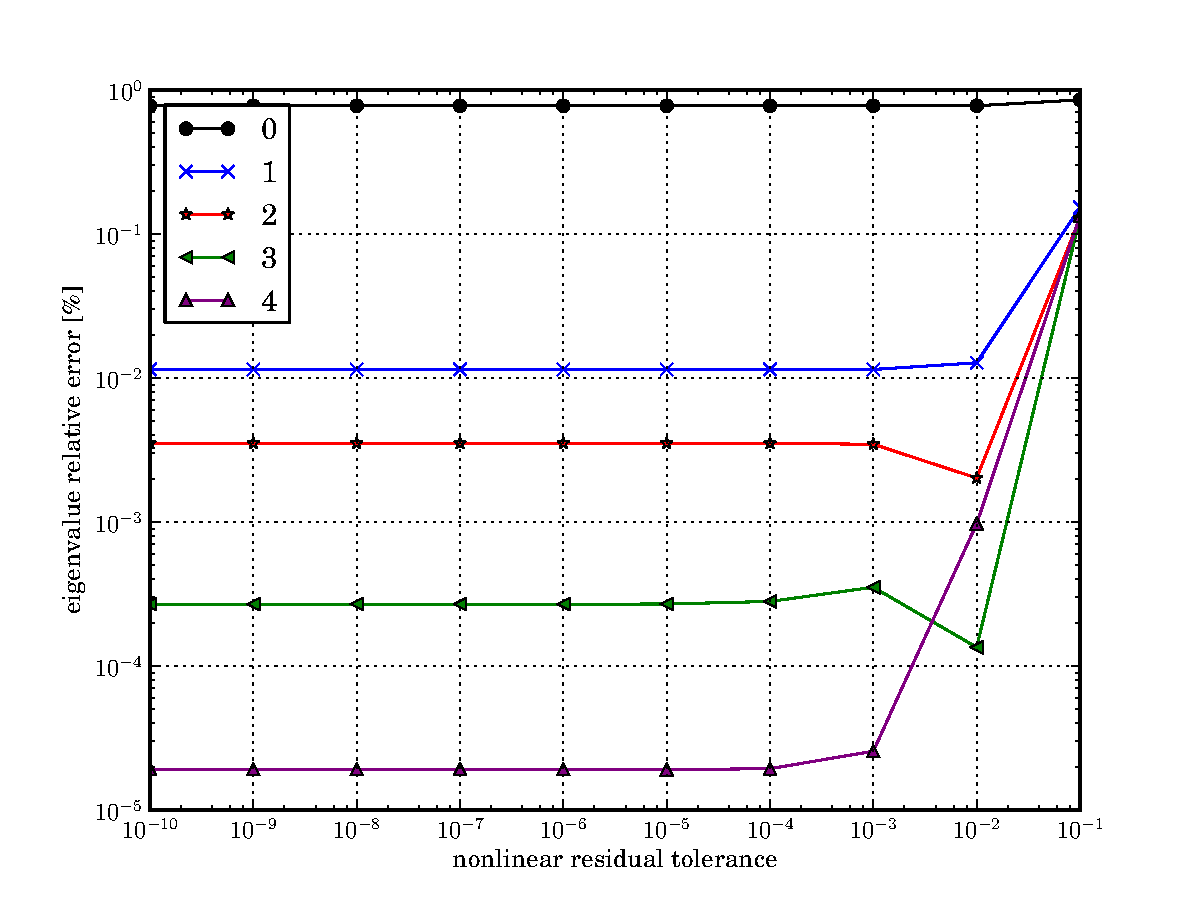
\includegraphics[keepaspectratio, width=1.0\textwidth]
                    {tolerance_study_eigenvalue}
    \caption{Eigenvalue error.}
    \label{fig:tolerance_study_eigenvalue}                   
  \end{subfigure}
  %
  \begin{subfigure}{0.49\textwidth}
    \centering
    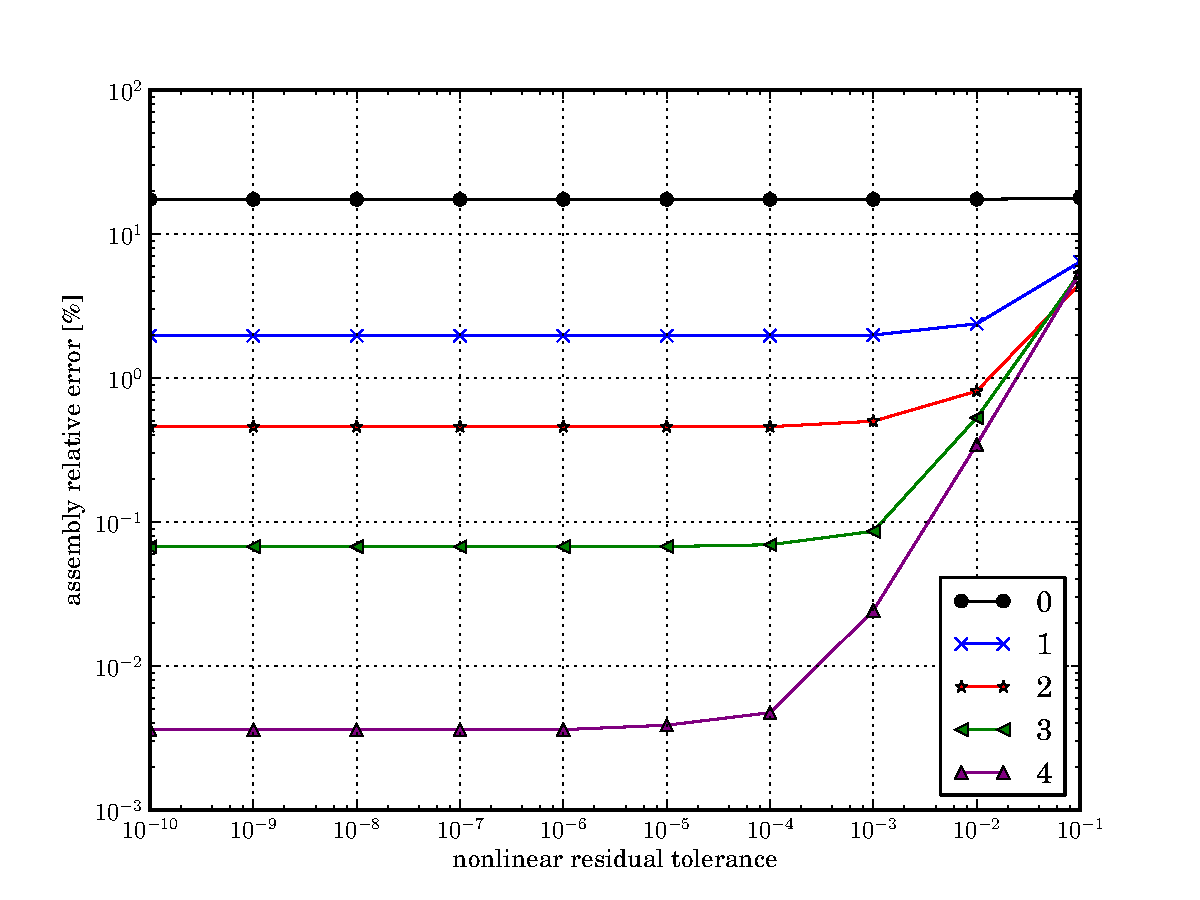
\includegraphics[keepaspectratio, width=1.0\textwidth]
                    {tolerance_study_power}
    \caption{Assembly power error.}
    \label{fig:tolerance_study_power}                 
  \end{subfigure}
  \caption{Absolute relative eigenvalue 
          (\ref{fig:tolerance_study_eigenvalue}) and 
          absolute maximum relative 
          assembly power
           (\ref{fig:tolerance_study_power})
          errors for the 2-D IAEA problem as functions of the
          residual norm tolerance for several spatial orders.}
  \label{fig:tolerance_study}
\end{figure*}

\subsubsection{Orders and Accuracy}
\label{sec:diffusion_order_accuracy}

While a detailed discussion of basis accuracies is outside the 
present scope, it is illustrative to assess convergence 
of the DLP spatial basis applied to the diffusion benchmarks.  
Figure \ref{fig:diffusion_order_study}
 shows the maximum relative error in the assembly 
powers and absolute relative eigenvalue error as functions of spatial order.
For the 
3-D IAEA problem, two approximations were used.  The first is a full 
expansion of order $m$ in both spatial variables, meaning that on a given 
side, the two-dimensional expansion is equivalent to the form 
\begin{equation}
 F(x, y) \approx a + bx + cy + d x^2 + e xy + f y^2 + \ldots \, .
\end{equation}
The second case uses an order reduction scheme that 
limits the sum of the $x$ and $y$ orders \cite{forget2006tdh}.  In this case,
\begin{equation}
 F(x, y) \approx a + bx + cy + d x^2 + f y^2 + \ldots \, ,
\end{equation}
where the cross term $e xy$ has been omitted.  Previous experience 
has demonstrated that these cross terms, particularly at high order, have 
little value, clearly demonstrated in Figure \ref{fig:diffusion_order_study}.

% Say something about the reduction in unknowns, the total node count, 
% etc.

For all the problems, a fourth order expansion yielded assembly 
(or nodal, for the IAEA-3D problem) errors below a tenth of a percent 
and eigenvalue errors on the range of a few pcm.  Consequently, a fourth 
order expansion was selected for use in comparing the solvers in 
subsequent performance analyses.

\begin{figure*}[htbp]
  \centering
  %
  \begin{subfigure}{0.49\textwidth}
    \centering
    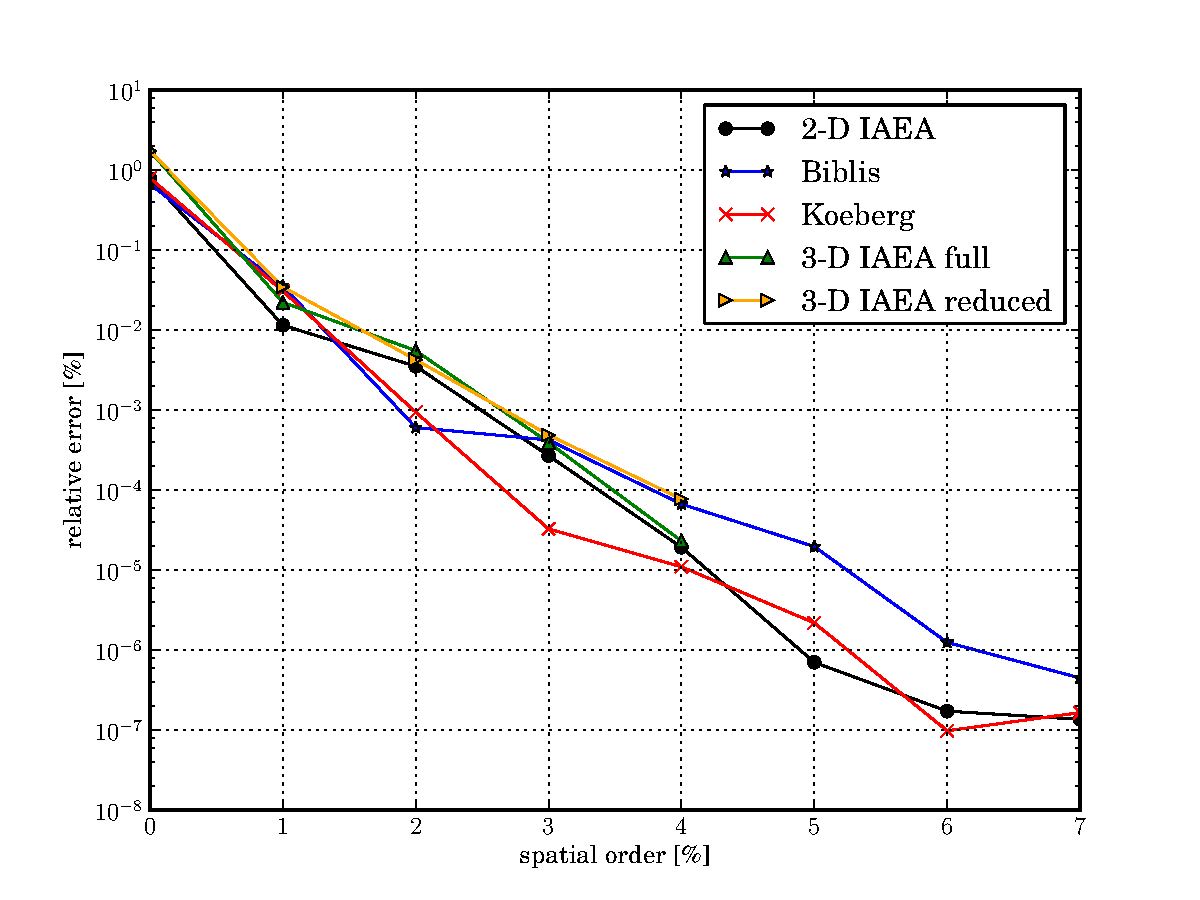
\includegraphics[keepaspectratio, width=1.0\textwidth]
                    {diffusion_order_study_eigenvalue}
    \caption{Eigenvalue error.}
    \label{fig:diffusion_order_study_eigenvalue}                   
  \end{subfigure}
  %
  \begin{subfigure}{0.49\textwidth}
    \centering
    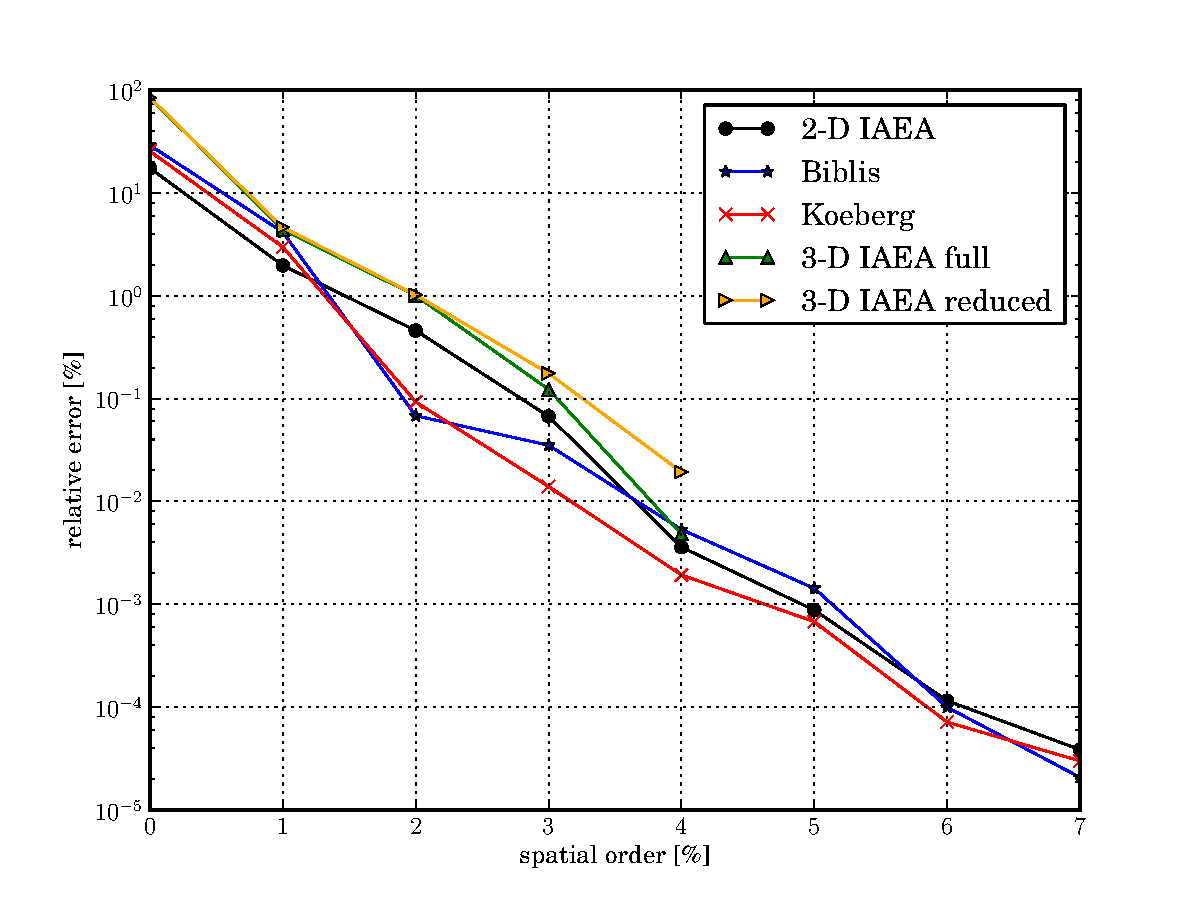
\includegraphics[keepaspectratio, width=1.0\textwidth]
                    {diffusion_order_study_power}
    \caption{Assembly power error.}
    \label{fig:diffusion_order_study_power}                 
  \end{subfigure}
  \caption{Absolute relative eigenvalue 
          (\ref{fig:diffusion_order_study_eigenvalue}) and 
          absolute maximum relative 
          assembly power
           (\ref{fig:diffusion_order_study_power})
          errors as functions of 
          spatial order.}
  \label{fig:diffusion_order_study}
\end{figure*}


\subsubsection{Inner Solver Comparison}

For the Picard solver, several eigenvalue solvers were investigated 
to solve the inner $\lambda$-eigenvalue problem, including the 
power (PI), Krylov-Schur (KS), and explicitly-restarted Arnoldi 
methods (ERAM), which are each
 implemented in SLEPc \cite{slepc}.  Because convergence of the 
outer Picard iteration is  sensitive to the inner convergence, 
the tolerance $\tau_{\lambda}$ of the inner problem was set 
more tightly at $10^{-10}$.  

Table \ref{tbl:diffusion_picard_inner_study} 
provides the number of inner and outer iterations,  total
computational time, and response generation time 
for each method and diffusion problem.
For all problems, 
KS outperforms ERAM by a small margin and PI by a factor of two 
or three.  Initial studies demonstrated that IRAM (not included 
by default with SLEPc) performs at about the same level 
as KS \cite{roberts2012ksi}. Were the tolerance smaller, the improvement 
of KS over PI would 
likely diminish.

For the three 2-D problems, the response time constituted a significant 
portion of the total computational time, ranging from about a third to half
depending on the solver.  For the 3-D IAEA problem, the global solver
was the dominant cost because the diffusion 
problems underlying the response generation are inexpensive compared to 
the much larger global problem.

\begin{table}[ht] 

 \begin{center} 
  \caption{Picard inner solver comparison for diffusion problems.} 
 \label{tbl:diffusion_picard_inner_study} 
 \begin{threeparttable}
 \begin{tabular}{ccccc} 
 \toprule 
  solver & time \tnote{a} & r. time \tnote{b} & inners & outers \\
 \midrule 
              &  \multicolumn{4}{c}{2-D IAEA} \\ 
 \midrule 
           PI &      1.87 &      0.37 &         3416 &            6 \\ 
           KS &      0.69 &      0.41 &           33 &            6 \\ 
         ERAM &      0.77 &      0.40 &           36 &            6 \\ 
 \midrule 
              &  \multicolumn{4}{c}{Biblis} \\ 
 \midrule 
           PI &      2.16 &      0.68 &         3437 &            5 \\ 
           KS &      0.97 &      0.68 &           31 &            5 \\ 
         ERAM &      1.05 &      0.69 &           34 &            5 \\ 
 \midrule 
              &  \multicolumn{4}{c}{Koeberg} \\ 
 \midrule 
           PI &      5.83 &      1.62 &         2012 &            3 \\ 
           KS &      2.38 &      1.66 &           21 &            3 \\ 
         ERAM &      2.63 &      1.67 &           21 &            3 \\ 
 \midrule 
              &  \multicolumn{4}{c}{3-D IAEA} \\ 
 \midrule 
           PI &    910.63 &     18.77 &         4427 &            6 \\ 
           KS &    210.91 &     19.47 &           75 &            6 \\ 
         ERAM &    294.48 &     19.75 &           70 &            6 \\ 
 \bottomrule 
 \end{tabular} 
 

 {\footnotesize
 \begin{tablenotes}
   \item[a] Total time [s]
   \item[a] Response generation time [s]
 \end{tablenotes}
 }
 \end{threeparttable}
 
 
 
 \end{center} 

\end{table} 


\subsubsection{Outer Solver Comparison}

Because KS outperformed the other inner solvers investigated, it was 
selected to study the Picard-based outer iteration schemes.
For this study, Picard iteration, along with the accelerated variant 
based on the {\it regula falsi} method, was compared to Steffensen's 
method and Newton's method.  

\subsubsection{Picard Acceleration}

The four Picard acceleration schemes were applied to the 2-D IAEA 
and Koeberg problems
using a fourth order expansion.  
Figure \ref{fig:diffusion_picard_acceleration}
shows the nonlinear residual as a function of outer iteration for the 
unaccelerated case along with the four accelerated cases. 

Picard iteration alone is a 
rapidly converging process, but acceleration schemes
can further reduce the number of iterations required.
Exponential and inverse-inverse extrapolation provide the 
most robust improvement, although for the Koeberg problem, 
they did not reduce the number of iterations.
The acceleration schemes each critically depend
on the limit $\lambda \to 1$, which is satisfied only if the responses are 
both conservative and computed very accurately.  The 
diffusion equation for each response is small and can be 
solved nearly exactly via LU factorization.  Moreover, the responses 
are conservative 
because a uniform mesh and DLP expansion were used. 
Even so, the linear-inverse and linear-linear suffered from their 
sensitivity to round-off errors, and even though care was taken when 
implementing the coefficients, the convergence tolerances used were 
not tight enough to ensure stability. Because the exponential 
scheme yielded a slightly smaller final residual norm, it was 
included for study with the remaining algorithms.
 
\begin{figure}[ht]
    \centering
    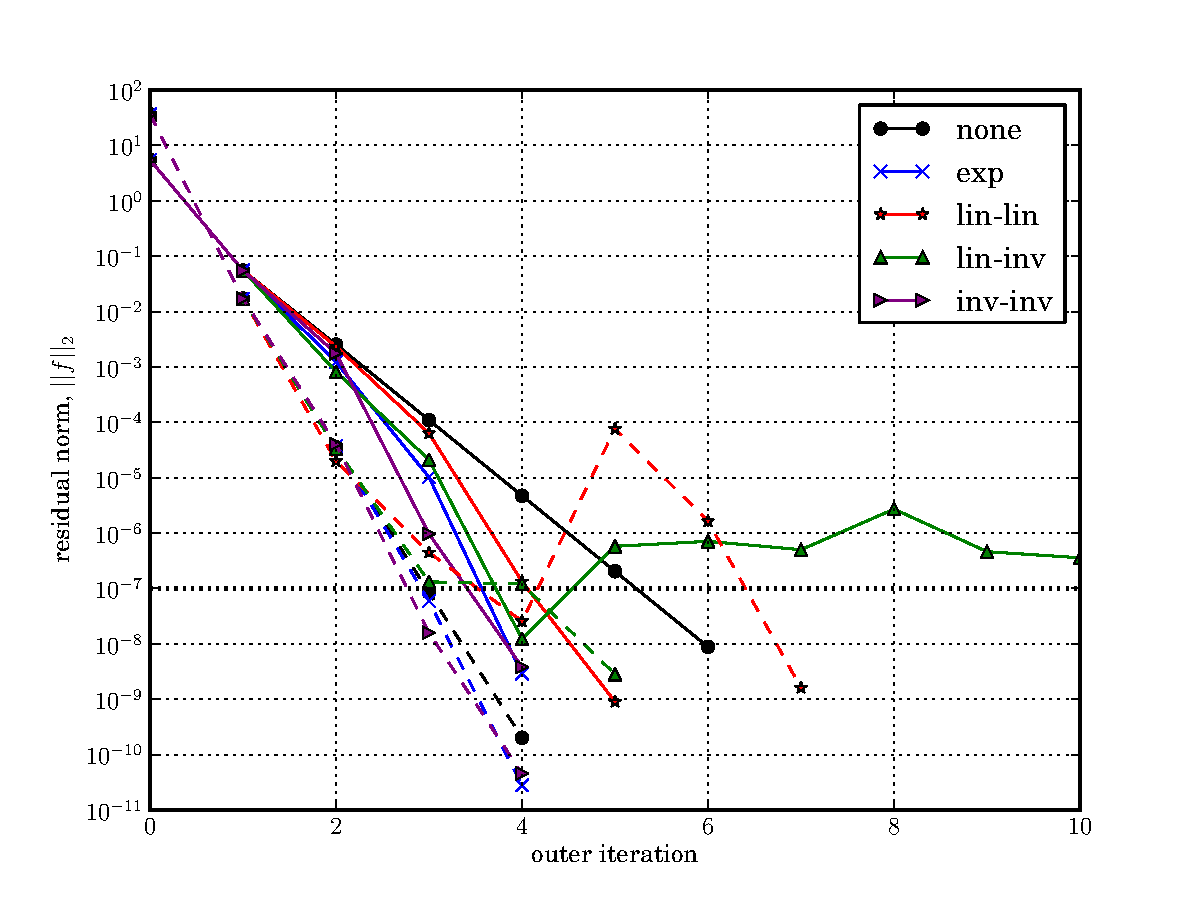
\includegraphics[keepaspectratio, width = 3.5 in]
                    {diffusion_picard_acceleration}
    \caption{Comparison of Picard acceleration schemes for the 
             2-D IAEA problem (solid lines) and Koeberg 
             problem (dashed lines).  }
    \label{fig:diffusion_picard_acceleration}
\end{figure}

\subsubsection{Newton Variants}

For Newton's method, unpreconditioned 
and preconditioned variants using ILU were studied.  The ILU preconditioner
is based on an explicit Jacobian constructed either once, using 
the initial responses, or every iteration, using the updated responses.  
In all cases, the underlying linear solves were performed with GMRES(30),
and the ILU preconditioner was applied with 0 through 2 levels.

Table \ref{tbl:diffusion_newton_pc_study} provides results for the 
2-D IAEA and Koeberg problems with a fourth order spatial 
expansion and $4\times 4$ nodes per assembly, corresponding to
184962 and 369922 unknowns, respectively.
Somewhat larger problems were used to highlight differences between
the preconditioners because the preconditioners offered no benefit 
for the single node case.

For both problems, ILU(0) preconditioning offered the best performance
with respect to time, although higher preconditioner levels 
led to lower numbers of inner iterations.
Failure to update the preconditioner had no discernible effect 
on the iteration count and yielded lower computational times than when 
the preconditioner was updated at every iteration.  This can be explained 
by noting that a majority of the Jacobian is relatively insensitive 
to small changes in $k$.  Given the initial guess for $k$ 
(unity in these cases)
is expected to be pretty close to the final answer, the original Jacobian
should be nearly equal to its final value.

\begin{table}[ht] 
 
 \begin{center} 
  \caption{Newton solver ILU preconditioner comparison for diffusion 
          problems.} 
 \label{tbl:diffusion_newton_pc_study}
 \begin{threeparttable}

 \begin{tabular}{ccccc} 
 \toprule 
  preconditioner & time\tnote{a} & r. time\tnote{b} & inners & outers \\
 \midrule 
 &  \multicolumn{4}{c}{2-D IAEA} \\ 
 \midrule 
          none &     12.62 &      0.46 &          477 &            4 \\ 
  no update ILU(0) &     10.43 &      0.46 &          144 &            4 \\ 
  no update ILU(1) &     11.68 &      0.46 &          118 &            4 \\ 
  no update ILU(2) &     12.37 &      0.46 &           86 &            4 \\ 
        ILU(0) &     10.69 &      0.46 &          144 &            4 \\ 
        ILU(1) &     14.07 &      0.45 &          118 &            4 \\ 
        ILU(2) &     17.12 &      0.45 &           86 &            4 \\ 
 \midrule 
 &  \multicolumn{4}{c}{Koeberg} \\ 
 \midrule 
          none &     45.82 &      3.29 &          403 &            4 \\ 
  no update ILU(0) &     43.18 &      3.34 &          157 &            4 \\ 
  no update ILU(1) &     52.18 &      3.35 &          136 &            4 \\ 
  no update ILU(2) &     58.26 &      3.35 &           91 &            4 \\ 
        ILU(0) &     45.61 &      3.35 &          157 &            4 \\ 
        ILU(1) &     67.44 &      3.38 &          136 &            4 \\ 
        ILU(2) &     89.90 &      3.35 &           91 &            4 \\ 
 \bottomrule 
 \end{tabular} 
 

 {\footnotesize
 \begin{tablenotes}
   \item[a] Total time [s]
   \item[b] Response generation time [s]
 \end{tablenotes}
 }
 \end{threeparttable}
 
 
 \end{center} 

\end{table} 

\subsubsection{Comparing Picard, Steffensen, and Newton}
\label{sec:global_solver_diffusion}

Several metrics can be used to compared the outer solvers. Ultimately, 
wall clock time is most important in practice.  However, the number of 
iterations 
of each method, both outer and inner, is also indicative of the 
algorithm performance, independent of any particular implementation.
These data are provided in Table \ref{tbl:diffusion_outer_study} 
for each of the benchmarks. A fourth
order spatial expansion  was used for all problems, with order reduction 
applied to the 3-D IAEA problem.  For the 2-D problems, a $4\times 4$ 
node-per-assembly model was used, while for the 3-D IAEA problem,  
a single node was used, corresponding to 184962 unknowns for the 
2-D IAEA and Biblis problems, 369922 for the Koeberg problem, 
and 988382 for the 3-D IAEA problem.

\begin{table*}[ht] 

 \begin{center} 
 
 \caption{Outer solver comparison for diffusion problems.} 
 \label{tbl:diffusion_outer_study} 
 
 \begin{threeparttable}
 \begin{tabular}{cccccc} 
 \toprule 
  solver & time\tnote{f}  & r. time\tnote{g} & inners & outers & $k$-evals. \\
 \midrule 
 &  \multicolumn{5}{c}{2-D IAEA} \\ 
 \midrule 
    P\tnote{a}        &     10.26 &      0.32 &           76 &            5 &            6 \\ 
    P+exp\tnote{b} &      9.09 &      0.27 &           65 &            4 &            5 \\ 
    S\tnote{c} &     11.20 &      0.39 &           80 &            3 &            7 \\ 
  N+$\delta k$\tnote{d} &     10.35 &      0.44 &          144 &            4 &            8 \\ 
  N+$\Delta k$\tnote{e} &     10.22 &      0.28 &          146 &            4 &            5 \\ 
 \midrule 
 &  \multicolumn{5}{c}{Koeberg} \\ 
 \midrule 
        P &      9.26 &      0.56 &           64 &            4 &            5 \\ 
    P+exp &      9.06 &      0.56 &           62 &            4 &            5 \\ 
    S &      9.36 &      0.56 &           64 &            2 &            5 \\ 
  N+$\delta k$ &     10.89 &      0.92 &          140 &            4 &            8 \\ 
  N+$\Delta k$ &     10.49 &      0.57 &          140 &            4 &            5 \\ 
 \midrule 
 &  \multicolumn{5}{c}{Biblis} \\ 
 \midrule 
    P &     25.65 &      1.61 &           54 &            3 &            4 \\ 
    P+exp &     25.76 &      1.62 &           54 &            3 &            4 \\ 
    S &     29.61 &      2.02 &           60 &            2 &            5 \\ 
  N+$\delta k$ &     43.10 &      3.26 &          157 &            4 &            8 \\ 
  N+$\Delta k$ &     42.07 &      2.05 &          157 &            4 &            5 \\ 
 \midrule 
 &  \multicolumn{5}{c}{3-D IAEA} \\ 
 \midrule 
        P &    213.51 &     17.93 &           75 &            6 &            7 \\ 
    P+exp &    167.93 &     12.79 &           62 &            4 &            5 \\ 
    S &    214.07 &     17.98 &           75 &            3 &            7 \\ 
  N+$\delta k$ &    269.36 &     20.93 &          129 &            4 &            8 \\ 
  N+$\Delta k$ &    261.27 &     13.02 &          129 &            4 &            5 \\ 
 \bottomrule 
 \end{tabular} 

 {\footnotesize
 \begin{tablenotes}
   \item[a] Picard 
   \item[b] Picard with exponential extrapolation
   \item[c] Steffensen
   \item[d] Newton with fine $k$ difference
   \item[e] Newton with coarse $k$ difference
   \item[f] Total time [s]
   \item[g] Response generation time [s]
 \end{tablenotes}
 }
 \end{threeparttable}
 
 \end{center} 
 
\end{table*} 

%  \footnote{fine finite difference for $k$}
%  \footnote{coarse finite difference for $k$}

The tested solvers include Picard (P) with and without exponential 
extrapolation (exp), Steffensen's method (S), and Newton's method (N).
For Newton's method, two schemes were examined.  The first is the same 
as used for testing the preconditioning and is based on a Jacobian with 
$k$-derivatives computed using a finite difference 
with a $\Delta k = 10^{-8}$.
The second scheme uses the two most recent $k$ values
for computing $\Delta k$, resulting in a larger $\Delta k$ and, therefore, 
a less accurate finite difference.  However, the accuracy of the finite 
difference did not affect the convergence, 
and for all four problems,
the coarse difference yielded the same number of outer iterations as the 
fine difference while reducing the number of $k$ evaluations by nearly half.

Steffensen's method provided the fastest convergence with respect to 
outer iterations, but it requires two $k$ evaluations per outer iteration.
Picard with exponential extrapolation yielded the lowest computational 
time and the fewest $k$ evaluations.  While Newton's method with a 
coarse $\Delta k$ is competitive with respect to $k$ evaluations, the 
overhead of solving the linear systems is higher than the cost of the 
$\lambda$-eigenvalue problem in the Picard iteration.

% FIGURE

\subsubsection{Comments}

Based on these diffusion analyses, Picard iteration with
KS for the inners and exponential extrapolation for accelerating 
the outers represents an ideal ERMM solver.  The Newton methods yield 
perform 
nearly as well with respect to $k$ evaluations, but the cost of 
applying the method is higher per iteration than the Picard variants,
implying further work on preconditioning the inner solves is warranted.

\subsection{2-D C5G7}

The 2-D C5G7 transport benchmark is a small quarter core 
model consisting of two UO$_2$ assemblies and two MOX
assemblies, all surrounded by an assembly-width reflector.  The model 
is based on 7 group data and homogenization of the fuel and cladding.
 
\subsubsection{Orders and Accuracy}
 
To assess the accuracy of the response schemes available for transport 
problems, the C5G7 benchmark was solved using a variety of 
angular bases. Because a uniform spatial mesh was 
not used, the DLP spatial expansion converged more slowly for 
the C5G7 problem than for the 
uniformly-meshed diffusion problems.  For all cases, 
the response transport calculations were converged to 
a relative residual norm of $10^{-8}$, and the outer calculation was 
converged to a nonlinear residual norm of $10^{-7}$.

Table \ref{tbl:c5g7_order_convergence} shows the convergence of 
the eigenvalue and pin power errors as a function of space-angle 
order.  By third order, the conservative basis yields
very limited improvement, most likely due to the DLP 
spatial basis used.  A nonuniform mesh yields a nonconservative
DLP expansion that is inaccurate at low orders compared to a
conservative expansion.
Table \ref{tbl:c5g7_order_convergence} shows that both the
DLP and Chebyshev bases yield
maximum relative pin power errors of slightly more than 2\%.
These results are in contrast to results reported in 
Ref. \cite{roberts2014psb}, 
which used a full order spatial basis to eliminate spatial errors and
showed that a conservative Chebyshev basis significantly outperforms a
DLP basis.
Consequently, the present results indicate that
spatial expansion errors are dominant by second or third order,
and, therefore, a full 
implementation and systematic study of new spatial bases 
is warranted.

\begin{table*}[ht] 
 
\begin{center} 

 \caption{2-D C5G7 order convergence.  All errors in \%, with 
          reference MCNP results from the original documentation.} 
 \label{tbl:c5g7_order_convergence} 

  \begin{threeparttable}
 \begin{tabular}{ccrrrrrr} 
 \toprule 
 basis & order & $e_k$\tnote{a}   & $\max |e_i|$\tnote{b}  & $ \frac{\max |e_i|}{p^{\text{ref}}_i} $  
   & $\frac{\sum_i |e_i|}{ N}$   &  $\frac{\sqrt{\sum_{i} e_{i}^2}}{N}$   
     & $ \frac{\sum_i |e_i|p^{\text{ref}}_i}{N} \bar{p}^{\text{ref}}$    \\
 \midrule 
 DLP-$\psi$  &    0  &     1.00   &    33.32   &   109.45   &     9.41   &     0.36   &    10.97   \\
 DLP-$\psi$  &    1  &     0.72   &    38.17   &    18.49   &     2.65   &     0.12   &     3.06   \\
 DLP-$\psi$  &    2  &     0.13   &     4.36   &     7.49   &     0.98   &     0.04   &     1.36   \\
 DLP-$\psi$  &    3  &     0.01   &     2.20   &     5.81   &     0.37   &     0.02   &     0.42   \\
 \midrule 
 Chebyshev-$\psi$  &    0  &     2.61   &    40.43   &   107.58   &     9.46   &     0.37   &    10.86   \\
 Chebyshev-$\psi$  &    1  &     0.07   &    19.93   &    11.38   &     0.99   &     0.05   &     1.22   \\
 Chebyshev-$\psi$  &    2  &     0.04   &     2.73   &     6.28   &     0.39   &     0.02   &     0.40   \\
 Chebyshev-$\psi$  &    3  &     0.04   &     2.27   &     6.00   &     0.35   &     0.02   &     0.38   \\
 \midrule 
 {\tt Detran}\tnote{c} & n/a  &     0.01   &     0.91   &     0.94   &     0.17   &     0.01   &     0.22   \\

% detran as reference
% DLP-$\psi$ &    0  &     1.00   &    33.35   &   108.87   &     9.49   &     0.36   &    11.11   \\
% DLP-$\psi$  &    1  &     0.72   &    37.78   &    18.52   &     2.63   &     0.12   &     3.07   \\
% DLP-$\psi$  &    2  &     0.13   &     4.67   &     7.74   &     0.92   &     0.04   &     1.25   \\
% DLP-$\psi$  &    3  &     0.01   &     2.35   &     6.24   &     0.35   &     0.02   &     0.37   \\
%  \midrule 
% Chebyshev-$\psi$ &    0  &     2.61   &    40.73   &   107.01   &     9.57   &     0.37   &    11.03   \\
% Chebyshev-$\psi$ &    1  &     0.07   &    19.54   &    11.09   &     1.01   &     0.06   &     1.26   \\
% Chebyshev-$\psi$ &    2  &     0.04   &     2.95   &     6.70   &     0.39   &     0.02   &     0.37   \\
% Chebyshev-$\psi$ &    3  &     0.04   &     2.42   &     6.43   &     0.35   &     0.02   &     0.35   \\
 \bottomrule 
 \end{tabular}  
 {\footnotesize
 \begin{tablenotes}
   \item[a] $e_k = |k-k^{\text{ref}}|/k^{\text{ref}}$  
   \item[b] $e_i = p_i - p^{\text{ref}}_i$, for $i$th pin
   \item[c] based on {\tt Detran} solution of the C5G7 problem with the same
            discretization and quadrature and, thus, represents the lower error 
            bound for {\tt Serment} 
 \end{tablenotes}
 }
 
 \end{threeparttable}
 
 \end{center} 

\end{table*} 

\subsubsection{Solver Comparison}

The same global solvers used in 
Section \ref{sec:global_solver_diffusion} were also applied 
to the 2-D C5G7 problem.  In this case, 64 processes were used 
for response generation, while a
single process was used for the outer ($\lambda$-eigenvalue) problem.

Table \ref{tbl:c5g7_outer_study} provides the wall time,
as well as the total and response time summed over all 
processes.  In addition, the number of inner iterations,
outer iterations, and $k$ evaluations are included. Newton's method with the 
coarse $k$ derivative yielded the best performance, with a wall 
time of $1.09\cdot 10^3$ seconds, total 
time of $6.97\cdot 10^4$ seconds (summed over 
all processes), and a solver (excluding response generation) time of 
$34$ seconds. Use of 
the fine $k$ derivative required more outer iterations and, consequently, 
significantly more time.  Steffensen's method required the 
fewest outer iterations but at the 
cost of more $k$ evaluations.  Standard Picard iteration 
readily converged, but extrapolation
failed miserably.  However, this failure is {\it completely expected}: 
the spatial basis is not conservative, so $\lambda$ does not 
tend toward unity, and, hence, extrapolation does not apply.  This 
highlights significant value in selecting a conservative basis, 
because the extrapolated Picard iteration was the best performing 
method for the diffusion problems.

\begin{table*}[ht] 
 \begin{center} 
 \caption{Outer solver comparison for 2-D C5G7 problem with first order expansions.
          Picard with exponential extrapolation fails due to the nonconservative spatial 
          basis, \ie $\lambda \ne 1$.} 
 \label{tbl:c5g7_outer_study} 
  \begin{threeparttable}
 \begin{tabular}{ccccccc} 
 \toprule 
  solver & w. time\tnote{f} & time\tnote{g} & r. time\tnote{h} & inners & outers & $k$-evals. \\
  \midrule
    P\tnote{a}            &  $1.67\cdot 10^3$ &  $1.07\cdot 10^5$ &  $1.07\cdot 10^5$ &           16 &            6 &            7 \\ 
    P+exp\tnote{b}        &  $6.26\cdot 10^3$ &  $4.00\cdot 10^5$ &  $4.00\cdot 10^5$ &           36 &           21 &           21 \\ 
    S\tnote{c}            &  $1.73\cdot 10^3$ &  $1.11\cdot 10^5$ &  $1.11\cdot 10^5$ &           16 &            3 &            7 \\ 
    N+$\delta k$\tnote{d}            &  $4.60\cdot 10^3$ &  $2.94\cdot 10^5$ &  $2.94\cdot 10^5$ &           76 &            8 &           16 \\ 
    N+$\Delta k$\tnote{e} &  $1.09\cdot 10^3$ &  $6.97\cdot 10^4$ &  $6.96\cdot 10^4$ &           33 &            4 &            5 \\ 
 \bottomrule 
 \end{tabular} 
 
 {\footnotesize
 \begin{tablenotes}
   \item[a] Picard 
   \item[b] Picard with exponential extrapolation
   \item[c] Steffensen
   \item[d] Newton with fine $k$ difference
   \item[e] Newton with coarse $k$ difference
   \item[f] Wall time [s]
   \item[g] Total time summed over all processes [s]
   \item[h] Total response generation time summed over all processes [s]
 \end{tablenotes}
 }
 
 \end{threeparttable}
 
 \end{center} 

\end{table*} 

\subsection{3-D Takeda}

The 3-D Takeda benchmark is a simple benchmark, but it
allows for in-depth examination of the convergence properties of 
the basis sets.  The model consists of three homogeneous regions using 
a two group approximation in energy.  For this study, the the ``rods in''
configuration was used.

\subsubsection{Order Convergence}

Figures \ref{fig:takeda_order_study_eigenvalue_error} and
\ref{fig:takeda_order_study_nodal_power_error} provide the absolute 
relative error in the eigenvalue and the maximum 
absolute relative error in the nodal powers as a function of angular 
order for several spatial orders.  Order reduction was used in 
both space and angle.  Very little improvement was observed
with increasing angular order for a spatial order of zero.  
For higher spatial orders, an increasing angular order 
yielded a monotonically decreasing error for both $k$ and the nodal 
powers.  The conservative basis outperformed the DLP variants, yielding
nearly sub-1\% nodal errors for a third order angular expansion and 
spatial orders greater than one.  DLP-$J$ yielded slightly 
better nodal powers than DLP-$\psi$ at higher orders but higher 
$k$ errors for all orders. 

For all angular bases, a significant trend observed was the markedly
diminishing returns for spatial orders above 
two.  In other words, the most consistent improvement observed,
irrespective of angular order and basis, was obtained by shifting 
from first to second order in space.  This trend is reasonable because 
the nodes are homogeneous, and boundary quantities should, therefore, 
be relatively smooth functions of space.

\begin{figure*}[htbp]
  \centering
  %
  \begin{subfigure}{0.49\textwidth}
    \centering
    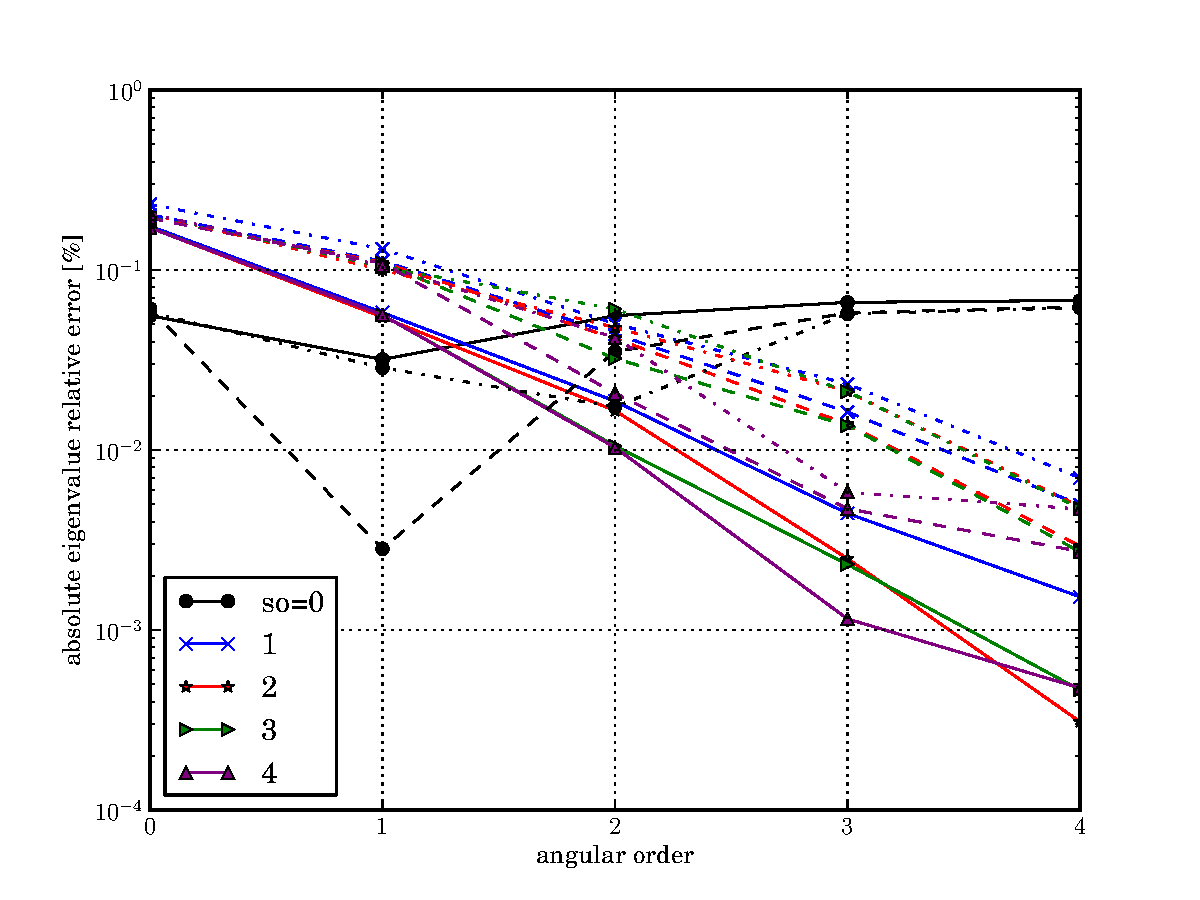
\includegraphics[keepaspectratio, width=1.0\textwidth]
                    {takeda_order_study_eigenvalue_error}
    \caption{Eigenvalue error.}
    \label{fig:takeda_order_study_eigenvalue_error}                   
  \end{subfigure}
  %
  \begin{subfigure}{0.49\textwidth}
    \centering
    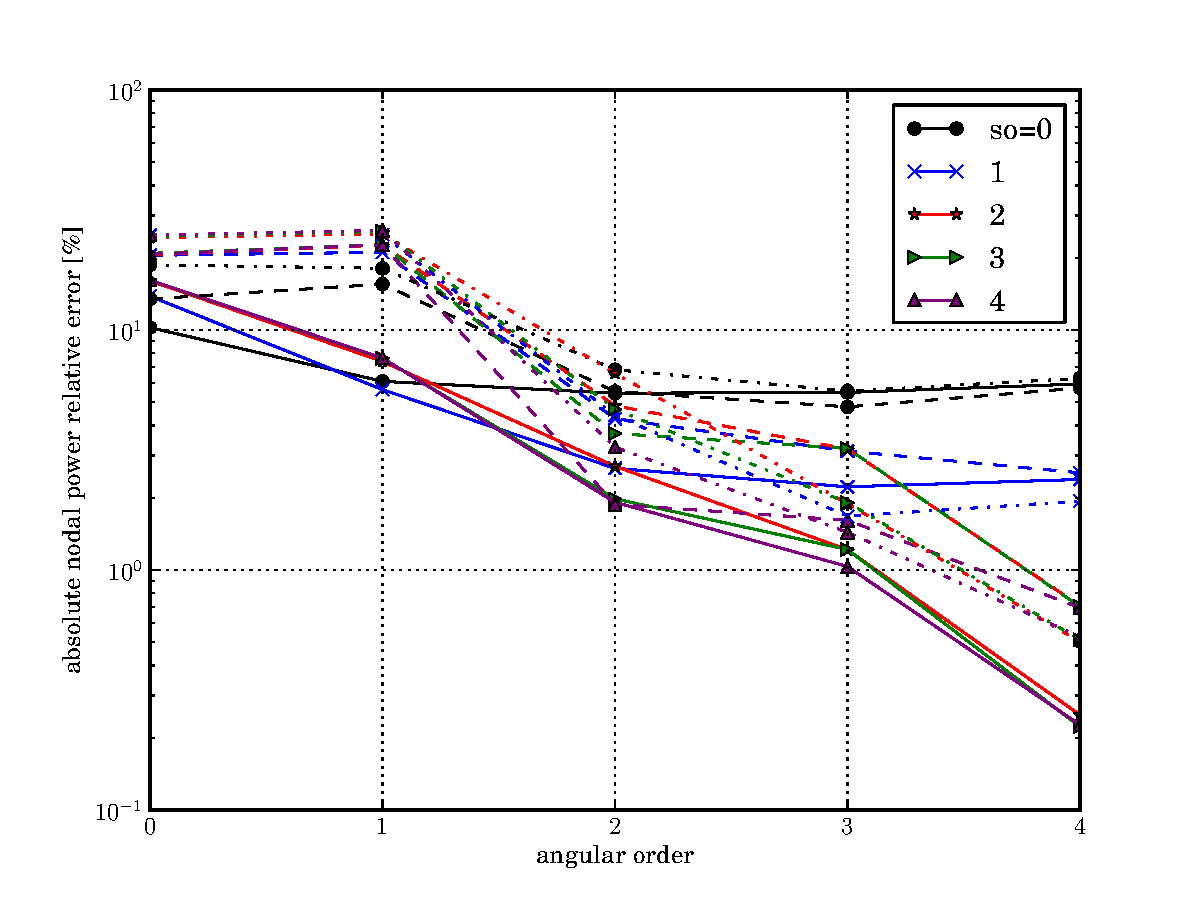
\includegraphics[keepaspectratio, width=1.0\textwidth]
                    {takeda_order_study_nodal_power_error}
    \caption{Nodal power error.}
    \label{fig:takeda_order_study_nodal_power_error}                 
  \end{subfigure}
  \caption{Takeda problem absolute relative 
           eigenvalue (\ref{fig:takeda_order_study_eigenvalue_error})
           and nodal power (\ref{fig:takeda_order_study_nodal_power_error})
           errors as 
           a function of angular order for several spatial orders.  
           The solid lines indicate the conservative basis, while the 
           dashed and dashed-dot lines indicate the DLP basis used to 
           expand the angular flux $\psi$ and current $J$, respectively.}  
  \label{fig:core_benchmark_plot}
\end{figure*}

\subsubsection{Solver Comparison}

The same solvers used for the diffusion  
and 2-D C5G7 problems were applied to the Takeda problem. A second 
order spatial expansion with a third order angular expansion in the 
azimuth and polar variables was used.  Order reduction was applied to 
the spatial and angular terms.  The problem was run with 64 processes, with 
one process for the global problem.  Table \ref{tbl:takeda_outer_study} 
provides the wall time, total time summed over all processors, and the 
total response function time summed over all processors.  

Similar to the diffusion results, the extrapolated Picard iteration 
proved to be the most efficient of the solvers studied.  
Newton's method with the coarse $k$ finite difference yielded just as 
few $k$ evaluations but with a slightly higher overall cost.

\begin{table*}[ht] 
 \begin{center} 
 \caption{Outer solver comparison for 3-D Takeda problem with second order 
          spatial expansion and third order polar and azimuthal angle 
          expansions.} 
 \label{tbl:takeda_outer_study} 
  \begin{threeparttable}
 \begin{tabular}{ccccccc} 
 \toprule 
  solver & w. time\tnote{f} & time\tnote{g} & r. time\tnote{h} & inners & outers & $k$-evals. \\
  \midrule
    P\tnote{a}            &  $9.76\cdot 10^2$ &  $6.25\cdot 10^4$ &  $5.91\cdot 10^4$ &           56 &           13 &           14 \\ 
    P+exp\tnote{b}       &  $3.51\cdot 10^2$ &  $2.24\cdot 10^4$ &  $2.12\cdot 10^4$ &           23 &        4 &   5  \\ 
    S\tnote{c}            &  $1.05\cdot 10^3$ &  $6.72\cdot 10^4$ &  $6.36\cdot 10^4$ &           58 &            7 &           15 \\ 
    N+$\delta k$\tnote{d}&  $7.30\cdot 10^2$ &  $4.67\cdot 10^4$ &  $4.26\cdot 10^4$ &           57 &            5 &           10 \\ 
    N+$\Delta k$\tnote{e}&  $3.87\cdot 10^2$ &  $2.48\cdot 10^4$ &  $2.14\cdot 10^4$ &           44 &          4 &           5  \\ 
 \bottomrule 
 \end{tabular} 
 
 
 {\footnotesize
 \begin{tablenotes}
   \item[a] Picard 
   \item[b] Picard with exponential extrapolation
   \item[c] Steffensen
   \item[d] Newton with fine $k$ difference
   \item[e] Newton with coarse $k$ difference
   \item[f] Wall time [s]
   \item[g] Total time summed over all processes [s]
   \item[h] Total response generation time summed over all processes [s]
 \end{tablenotes}
 }
 
 \end{threeparttable}
 
 \end{center} 
\end{table*} 

\section{Conclusion}
\label{sec:conclusion}

Based on the results for both the diffusion and transport problems, Picard 
iteration with exponential extrapolation appears to be the most
efficient method studied, yielding minimum numbers of $k$ evaluations 
while providing the lowest global solver overhead.  However,  
extrapolation is based on $\lambda$ converging to unity, and because this 
is not always guaranteed, Newton's method with the coarse finite difference 
provides a more consistently robust solver, with nearly as 
few $k$ evaluations and only relatively small overhead due to the 
inner linear solves.

Further work on preconditioners for Newton's method 
will likely reduce the corresponding (global) computation time 
to levels similar to extrapolated Picard iteration.  
Even so, the efficacy and 
simplicity of Picard iteration suggests that care should be taken to 
select a conservative basis leading to $\lambda = 1$ upon convergence.

Ultimately, the present work supports broader efforts to use 
ERMM for production level analyses, but significant challenges remain,
dominated by the vast number of responses required for realistic 
modeling.  Solvers were developed that reduce the number of $k$ evaluations 
required and minimize time spent generating  
responses, while related recent work successfully developed diffusion-based 
transport preconditioners that significantly reduce the time of 
individual response calculations \cite{roberts2014dpm}.  Because 
responses are independent, parallel computation will be a natural
component of 
any future ERMM implementation.  Scoping studies have demonstrated 
nearly ideal scaling of {\tt Serment} on a small research 
cluster \cite{roberts2014arm}, and ongoing work aims to test {\tt Serment} on 
leadership-class machines.

\section*{Acknowledgements}

The work of the first author was supported in part by a
Department of Energy Nuclear Energy University Programs Graduate Fellowship.
Additionally, the authors wish to thank one of the reviewers
for comments that helped clarify aspects of the early response 
matrix literature.


%% References with bibTeX database:
\bibliographystyle{elsarticle-num}
\bibliography{robertsj_thesis.bib}
%\bibliographystyle{unsrt}


\end{document}

\begin{abstract}

\end{abstract}

%-------------------------------*- Mode:TeX -*-------------------------------%
\section{Introduction and Background}
\label{sec:litreview}

Fundamental to reactor modeling is analysis of the steady-state 
balance of neutrons, described concisely as
\begin{equation}
  \oper{T} \phi(\vec{\rho}) = \frac{1}{k} \oper{F} \phi(\vec{\rho}) \, ,
  \label{eq:global}
\end{equation}
where the operator $\oper{T}$ describes transport processes, $\oper{F}$ 
describes neutron generation, $\phi$ is the neutron flux, $\vec{\rho}$ 
represents the relevant phase space, and $k$ is the eigenvalue, the ratio 
of the number of neutrons in successive generations. 

Since the late 1970's, full core analyses for light water reactors 
(LWR) have been performed using relatively low fidelity nodal methods 
based on clever homogenization of phase-space with proven success.  
However, as current reactors become increasingly heterogeneous 
due more aggressive fuel loadings and longer 
cycle lengths in existing LWR's, nodal methods are becoming less applicable, 
and for new, highly heterogeneous reactor designs, even less so. Although 
advances in production nodal codes, including use of generalized multigroup 
SP$_3$ transport with subassembly resolution, address issues related
to more complicated designs \cite{bahadir2009sng}, there likely is limited 
room for further improvement of the underlying approach.
Consequently, a move toward full core analysis techniques that can 
leverage the high fidelity methods typically used for smaller problems 
is desired.  


%============================================================================%
\subsection{The Eigenvalue Response Matrix Method}

One such approach is the response matrix method (RMM), which is 
based on a spatial decomposition of the global problem of Eq. \ref{eq:global}
into local fixed source problems connected by approximate boundary
conditions.
The response matrix method has been used in various forms since 
the early 1960's \cite{shimizu1963arm}.  Using the terminology of 
Lindahl and Weiss \cite{lindahl1981rrm}, the method can be formulated 
using explicit volume flux responses, called the ``source'' RMM, or by 
using current responses that include fission implicitly and hence are 
functions of $k$, known as the ``direct'' RMM.  Although both forms are 
used in various nodal methods, the source RMM is more widespread. 
This work is on the the direct RMM, which shall be referred to as the 
{\it eigenvalue} response matrix method (ERMM).

Several formulations of ERMM have been proposed since its first use in 
the 1960's. Here, a rather general approach is described based 
on expansions of the boundary conditions that couple
subvolumes of the global problem, a formalism introduced 
as early as the work of Lindahl \cite{lindahl1976mdr} and
studied more recently by several authors
\cite{mosher2006ifr, roberts2011ser, roberts2012ksi}.  

Suppose the global problem 
of Eq. \ref{eq:global} is defined over a 
volume $V$.  Then a local homogeneous problem can be defined over a 
subvolume $V_i$ subject to 
\begin{equation}
  \oper{T} \phi(\vec{\rho}_i) = 
    \frac{1}{k} \oper{F} \phi(\vec{\rho}_i) \, ,
  \label{eq:local}
\end{equation}
and
\begin{equation}
  J^{\mathrm{local}}_{-} (\vec{\rho}_{is}) = 
    J^{\mathrm{global}}_{-}(\vec{\rho}_{is}) \, ,
  \label{eq:localbc}
\end{equation}   
where $J^{\mathrm{local}}_{-} (\vec{\rho}_{is}) $ is a 
function of the incident boundary flux, typically the 
partial current, which quantifies net flows through a 
surface.

To represent the local problem numerically, an orthogonal basis, $P_n$,
over the relevant phase space is defined
\begin{equation}
  P_n(\vec{\rho}_{is}), \,\,\, n = 0, \, 1, \, \ldots N  \\
\end{equation}
subject to
\begin{equation}
   \int P_m(\vec{\rho}_{is}) P_n(\vec{\rho}_{is})  d\rho_{is}
     = \delta_{mn} \, .
\end{equation}
A response equation is defined 
\begin{equation}
 \oper{T} \phi_{i}^{ms} (\vec{\rho}_i) = 
   \frac{1}{k} \oper{F} \phi_{i}^{ms} (\vec{\rho}_i) 
\end{equation}
subject to
\begin{equation}
 J^{\mathrm{local}}_{-} (\vec{\rho}_{is}) = P_m(\vec{\rho}_{is}) \, .
\end{equation}
The resulting outgoing currents $J_{-} (\vec{\rho}_{is}) $ are used to define
response functions
\begin{equation}
       r^{ms}_{im's'} = \int  P_{m'}(\vec{\rho}_{is'})  
        J_{i+}^{m} (\vec{\rho}_{is'}) d\rho_{is'} \, .
\label{eq:responsefunction}
\end{equation}
The quantity $r^{ms}_{im's'}$ has a simple physical
interpretation: it is the $m'$th order response 
out of surface $s'$ due to a unit incident $m$th order condition on 
surface $s$ of subvolume $i$. 

The incident and outgoing currents are expressed as
truncated expansions using the same basis
\begin{equation}
  J_{is\pm}(\vec{\rho}_{is}) \approx \sum^{N}_{n=0}  
    j^n_{is_\pm} P_n (\vec{\rho}_{is}) 
\end{equation}
where
\begin{equation}
      j^n_{is_\pm} = \int  P_n (\vec{\rho}_{is}) 
        J_{\pm} (\rho_{is}) d \rho_{is} \, .
\end{equation}
These coefficients are then represented in vector form as
\begin{equation}
  \mathbf{J}_{i\pm} = ( j^0_{i1_\pm} \, j^1_{i1_\pm} \, \ldots \, 
    j^0_{i2_\pm} \, j^1_{i2_\pm} \, \ldots \, j^N_{iS_\pm} )^\mathsf{T} \, ,
\end{equation}
and using these together with Eq. \ref{eq:responsefunction} yields
the nodal balance equation
\begin{equation}
    \mathbf{J}_{i+} = 
%     \left [\begin{array}{c}
%       j^0_{i1_+}    \\
%       j^1_{i1_+}    \\
%       \vdots        \\
%     \end{array} 
%     \right ] =
     \left [\begin{array}{ccc}
       r^{01}_{i01} &  r^{11}_{i01}  &  \cdots   \\
       r^{01}_{i11} &  r^{11}_{i11}  &  \cdots   \\
                    &                &  \ddots   \\
    \end{array} 
    \right ] \left [\begin{array}{c}
      j^0_{i1_-}       \\
      j^1_{i1_-}       \\
      \vdots           \\
    \end{array} 
    \right ] = \mathbf{R}_i\mathbf{J}_{i-} \, .
  \label{eq:elementresponse}
\end{equation}

Global balance is defined by the eigenvalue response matrix
equation
\begin{equation}
  \oper{M}\mathbf{R}(k)\mathbf{J_-}  = \lambda \mathbf{J_-} \, ,
  \label{eq:erme}
\end{equation}
where 
$\oper{R}$ is the block diagonal response matrix of $\oper{R}_i$,  
$\mathbf{J}_{-}$ are vectors containing all incident current coefficients, 
$\oper{M}=\oper{M}^\mathsf{T}$ is 
the connectivity matrix that redirects outgoing responses as incident
responses of neighbors, superscript $\mathsf{T}$ represents the matrix 
transpose, and $\lambda$ is an eigenvalue that
represents the global balance of neutron currents through all 
nodal surfaces.
If the response matrix $\oper{R}$ is conservative (i.e. it
strictly maintains neutron balance),
\begin{equation}
 \lim_{k\to k^*} \lambda = 1 \, ,
\end{equation}
where $k^*$ is the true eigenvalue.
For nonconservative response expansions, the deviation of $\lambda$ from
unity measures discontinuities introduced across node boundaries and 
may be used to evaluate accuracy of the expansions used (with 
respect to an infinite expansion).


The $k$-eigenvalue can be interpreted physically as the ratio of neutrons
produced in one generation to the previous generation. 
Alternatively, $k$ can be viewed as the ratio of gains to losses in a given 
generation, and when applying this interpretation to the response matrix 
formalism, $k$ can be updated via the process
\begin{equation}
  k_{n+1} = \frac{\mathbf{F}(k_{n})\mathbf{J}_{-}} 
  { \mathbf{A}(k_{n}) \mathbf{J}_{-} + \mathbf{L}(k_{n}) \mathbf{J}_{-} }\, ,
\label{eq:picard}
\end{equation}
where $\oper{F}(k)\mathbf{J}_{-}$ is the global fission rate, 
$\oper{A}(k) \mathbf{J}_{-}$ is the global absorption rate,
and $\oper{L}(k) \mathbf{J}_{-}$ is the total leakage rate
from global boundaries.

%===========================================================================%
\subsection{Survey of ERMM Implementations}

The method defined by Eqs. \ref{eq:local}-\ref{eq:picard}
originates from the work of Shimizu et al. 
\cite{shimizu1963rmm, shimizu1963arm}, which appears to be the first work 
on response matrix methods (although the authors acknowledged a 
connection between their work and the earlier and more general 
theory of invariant imbedding as developed by Bellman et al. 
\cite{bellman1960iim}).  The method was originally based on 1-D diffusion 
in slab geometry. Aoki and Shimizu extended the approach to two dimensions, 
using a linear approximation in space to represent boundary
currents \cite{aoki1965arm}.
A shortcoming of this early work was an assumed value (unity) of 
the $k$-eigenvalue when evaluating responses, following which 
Eqs. \ref{eq:erme} and \ref{eq:picard} were solved just once 
to compute $k$.
Typically $k \approx 1$ for nuclear reactors, so the errors observed 
were only tens of pcm, which may have been deceptively small
and not representative of more general cases.  
In the later 2-D analysis \cite{aoki1965arm}, the results compared 
favorably to fine mesh diffusion calculations.

Weiss and Lindahl generalized ERMM by considering arbitrarily 
high order expansions of the boundary currents in Legendre 
polynomials \cite{weiss1975hor} and introducing an 
iterative sceheme for the $k$-eigenvalue equivalent to Eq. \ref{eq:picard}.
Lindahl also studied expansions of the current, comparing Legendre 
expansions to an approach that divides the boundary in several segments 
in which the current is assumed flat \cite{lindahl1976mdr}.  A more
complete overview of these approaches can be found in the review by Lindahl
and Weiss \cite{lindahl1981rrm}.

These diffusion-based methods rely on semi-analytic solutions to the 
diffusion equation and hence require homogeneous nodes. Previous 
scoping studies examined diffusion-based responses using discretized 
operators \cite{roberts2011ser}.  By numerically integrating the diffusion 
equation, heterogeneous nodes are treated naturally, though no diffusion 
models with heterogeneous nodes were studied.


In addition to methods based on diffusion theory, previous work applied 
transport theory for generating responses. Pryor et al. used 
a hybrid stochastic-deterministic approach based on
Monte Carlo and the collision probability 
method to generate responses \cite{pryor1973rmm, pryor1975rdr,
sicilian1975atr}.  Their work is unique in its definition
of the response matrix $\oper{R}(k)$ based on a precomputed 
series expansion.  Considering again Eq. \ref{eq:local}, the 
solution $\phi$ (omitting 
indices) can
be expressed as
\begin{equation}
 \phi = \phi_{0} + \frac{1}{k}\phi_{1}
                 + \frac{1}{k^2}\phi_{2}  + \ldots \, ,
\end{equation}
where $\phi_{i} $ is the flux for the $i$th neutron
generation due to fission.  The 
associated responses can be similarly defined
\begin{equation}
 \oper{R}(k) = \oper{R}_0 + \frac{1}{k}\oper{R}_1
                 + \frac{1}{k^2}\oper{R}_2  + \ldots \, .
\label{eq:responsesum}
\end{equation}
The authors claim this series can be truncated in as few as three terms 
by estimating the analytical sum, though the accuracy is not 
specified \cite{sicilian1975atr}.  When no fissile material is present, 
$\phi_{i} = 0$ for $i > 0$, and so $\oper{R}(k) = \oper{R}_0$.


A somewhat similar approach was developed by 
Moriwaki et al. \cite{moriwaki1999ndc}
in which Monte Carlo is used to 
generate assembly-level responses for full core analyses. 
Their method decomposes the response
matrix into four physically distinct components: 
transmission of incident neutrons from one surface to another surface ($T$), 
escape of neutrons born in the volume out of a surface ($L$), 
production of neutrons in the volume due to neutrons born in the 
volume ($A$), and production of neutrons in the volume due to neutrons 
entering a surface ($S$). If all indices but the 
surface are neglected, a current response can be expressed as
\begin{equation}
 r^{s}_{t} = T^s_t + \frac{1}{k}S^s(L_t + \frac{1}{k}A(L_t 
                   + \frac{1}{k}A(L_t + \cdots )) + \cdots) \, .
\label{eq:responseiterate}
\end{equation}
Like Eq. \ref{eq:responsesum}, this infinite sum 
represents the contributions of each generation to the 
total response.  The
matrices $\mathbf{T}$, $\mathbf{L}$, $\mathbf{A}$, and $\mathbf{S}$ 
are precomputed, and the full matrix $\mathbf{R}$ is
computed on-the-fly by iteration.  In the actual implementation, the 
volume-dependent responses are unique for each pin in an assembly.  
Additionally, spatial segmentation is used on boundaries, but angular 
dependence is neglected.

The more recent extension of Ishii {\it et al.} improved the 
angular accuracy by including angular segmentation. 
However, the resulting amount of data required
is quite significant, since the responses are then
dependent on spatial segment, angular segment, energy
group, and for volume responses, unique pins.
Therefore,  the approach in Eq. \ref{eq:responsesum} may be more 
economical because no volume-dependent responses are required.
However, computing pin reaction rates would still require 
volume-dependent responses but would preclude their use in 
solving Eq. \ref{eq:erme}.

Other related work has been development of the incident
flux expansion method \cite{mosher2006ifr,ilas2003hcm}. 
Initial work by Ilas and Rahnema focused on a variational
approach using a basis of Green's functions
for each variable with one-dimensional discrete 
ordinates \cite{ilas2003hcm}.  Mosher and Rahnema extended the 
method to two dimensions using discrete Legendre polynomials 
for space and angle expansions.  In addition, they
introduced a nonvariational variant that is equivalent to ERMM, but 
without explicit construction of matrices.  Forget and Rahnema
 extended this nonvariational approach to
three dimensions using Monte Carlo  with continuous
Legendre polynomials in space and angle \cite{forget2006tdh}.
In all cases, the responses were precomputed as functions
of the $k$-eigenvalue, and linear interpolation was
used to compute responses during global analysis.

\subsection{Major Challenge}

The application of ERMM to realistic steady-state analyses with 
feedback effects entails several challenges, predominantly 
the shear number of responses functions and hence transport solves
required.  These response functions are entirely independent
for a given state and $k$, making ERMM ideal for parallelization.

In the past work on ERMM, responses were precomputed as a function of 
$k$ and interpolated as needed.  In many cases, clever use of symmetry 
can reduce the amount of required data.  For benchmark problems, this
reduction is helpful, but as the effects of thermal feedback are included, 
each node becomes unique and, usually, asymmetric.  As such, precomputation 
of responses would require inclusion of dependence on several variables
in addition to $k$.
There seems at this time no completely satisfactory way to parameterize 
a response function database for accurate steady-state analyses.  
Parameterization becomes even more difficult if burnup is included 
for cycle analyses. Recent work has attempted to parameterize the 
responses for steady-state analysis of cold critical 
experiments \cite{hino2012bwr}.  While the results
are promising (sub-percent errors on pin fission rates), the problem 
assessed is not entirely representative of the current problems of interest.
Consequently, this paper focuses on ERMM implementations suitable for 
online generation of response functions because, at present, this appears 
to be the only meaningful manner in which to apply ERMM.  However, any
improvements developed for online response generation would be readily 
applicable to generation of response databases should an adequate 
parameterization scheme be developed in the future.

%============================================================================%
\subsection{Goals}

The primary goal of this work is to develop a response matrix method that
can efficiently leverage high fidelity deterministic transport methods for 
solving large-scale reactor eigenvalue problems on a variety of computer 
architectures.  
% Once the responses defining Eq. \ref{eq:erme} are defined, an 
% iterative scheme is 
% required to solve for the boundary coefficients and eigenvalue.  The most
% common approach historically has been to use the power method to solve the 
% global balance equation for $J$, with a corresponding $k$-update 
% based on neutron balance, leading to a fixed point iteration.  
% Within this fixed point iteration, more efficient schemes can be 
% used to solve the global balance equation.  
% However, in practice the most expensive part of the computation is likely 
% to be the response functions.  If these are computed on-the-fly (that is, 
% for each new $k$), a method that minimizes the number of $k$ evaluations is
% highly desirable.
Several solvers that support this goal are developed in this paper,
which substantially extends and elaborates on the authors' 
previous work \cite{roberts2011ser, roberts2012ksi}, and
the remainder of which is organized as follows.
 Section \ref{sec:inner}
discusses solution of the response matrix equations via fixed point 
iteration and methods for solving the resulting eigenvalue problem 
for $\lambda$ efficiently.  Section \ref{sec:outer} presents schemes 
that provide faster convergence in $k$ than standard fixed-point iteration,
which is important because the number of $k$-evaluations defines the 
number of responses evaluated.  A numerical study 
of the methods applied to several benchmark problems is 
provided in Section~\ref{sec:results}, followed by concluding remarks in
Section~\ref{sec:conclusion}.


%----------------------------------------------------------------------------%
\section{Solving the $\lambda$-Eigenvalue Problem}
\label{sec:inner}


Equations \ref{eq:erme} and \ref{eq:picard} represent
a Picard (fixed point) iteration
for the $k$-eigenvalue.  For each new $k$ value, however, the 
$\lambda$-eigenvalue problem defined by Eq. \ref{eq:erme} must be 
solved.

Historically, the method to solve Eq. \ref{eq:erme} is equivalent to 
simple power iteration.
For a given $k^{(n)}$, the current vector $\mathbf{J}_{-}$ is 
initialized,
$\mathbf{MR}(k^{n})$ is applied to the $\mathbf{J}_{-}$, and the resulting 
vector points closer to the dominant eigenvector of interest.  
The process repeats until converged. 

Unfortunately, the asymptotic convergence rate to the dominant mode is 
equal to $\ln{(1/\rho)}$, in which the dominance ratio $\rho$  is defined
\begin{equation}
 \rho = |\lambda_2| / |\lambda| \, ,
\end{equation}
and the eigenvalues of 
$\mathbf{M}\mathbf{R}$ satisfy 
$\lambda > |\lambda_2| \geq |\lambda_i| \, , \,\,\, \forall \, i > 2$.  
For many problems, $\rho$ typically falls 
above $0.99$ and is frequently larger than the dominance 
ratio associated with $k$.

Because of the large dominance ratio, 1000's of iterations are required 
to reduce residual norms $||\mathbf{MRJ}_- - \lambda \mathbf{J}_-||$ to 
within the tolerances typically employed. 
Chebyshev acceleration 
has been considered for accelerating convergence, but its utility is severely 
limited due to the eigenspectrum of $\mathbf{MR}$, a 
significant portion of which sits away from the real axis.  
For a representative problem, previous work 
showed that the expected (theoretical) speedup is limited to 
approximately two, compared to the factor of 20 gained if the spectrum is
completely real \cite{roberts2012ksi}.
Despite these theoretical limitations, 
Chebyshev acceleration has been used successfully for solving the inner 
problem \cite{zhang2012ehs}.  However, such success is likely highly 
problem-dependent and subject to significant tuning.

Alternatively,
more efficient eigenvalue solvers such as Krylov subspace 
methods can be used for the $\lambda$-eigenvalue problem.  
Krylov methods are based on generation
of a Krylov subspace of dimension $n$, 
defined for an $m \times m$ operator $\oper{A}$ as
\begin{equation}
 \mathcal{K}(n,x_0) \equiv \text{span} 
     \{x_0,\, \oper{A}x_0,\, \oper{A}^2x_0 , \, 
        \ldots , \, \oper{A}^{m-1}x_0 \} \, , 
 \label{eq:krylovsubspace}
\end{equation}
for some initial, possibly random, vector $x_0$.  The fundamental 
goal of all Krylov subspace methods is to find  $x \in \mathcal{K}(n,x_0)$  
that ``best'' solves the system of interest, be it an 
eigenproblem or linear system, where it is assumed that $n \ll m$.

Using $\mathcal{K}(n, x_0)$ directly is difficult numerically because
repeated application of $\oper{A}$ sends the initial vector $x_0$ into the
same direction, namely that of the dominant eigenvector of $\oper{A}$.  
Hence, the basis 
must be orthogonalized. The canonical approach for nonsymmetric 
operators is Arnoldi's method, which by successive application of the 
modified Gram-Schmidt process yields the Arnoldi decomposition
\begin{equation}
 \oper{A}\oper{V} = \oper{V} \oper{H} + fe^{\transp}_n \, ,
\end{equation}
where $\mathbf{V} \in \mathbb{R}^{m\times n}$  consists of
orthonormal columns,
$\mathbf{H} \in \mathbb{R}^{n \times n} $ is an upper Hessenberg matrix, 
$e_n$ is a zero vector with its last entry equal to one, and $f$ is 
the residual, which is orthogonal to the columns of $\mathbf{V}$.  

The eigenvalues of $\mathbf{H}$, called {\it Ritz values}, tend to
be good estimates of eigenvalues of $\mathbf{A}$, and given an eigenpair
$(\tilde{\lambda}, y)$ of $\mathbf{H}_n$, the Rayleigh-Ritz estimate of the
corresponding eigenvector of $\mathbf{A}$ is defined $x = \mathbf{V}_n y$ and
is called a {\it Ritz vector}.  Using these approximate 
eigenvalues and eigenvectors is the basis of Arnoldi's method.

The eigenpairs of $\oper{H}$ are found via a dense eigensolver, such as 
the QR method.  While these dense problems are small (since $n \ll m$), 
they are solved repeatedly for increasing $n$ until converged.  
If $n$ becomes too large, the dense methods become too expensive.  A 
more efficient approach is to restart Arnoldi's method. In 
the {\it explicitly} restarted Arnoldi method (ERAM), some combination of 
the existing $n$ Ritz vectors is used to choose a single starting guess, 
from which a new Arnoldi factorization is generated \cite{slepc}.
An alternative to explicit restart is {\it implicit} restart, where the 
desired portion of the spectrum is retained continuously by contracting 
from a subspace of dimension $n$ to a smaller space of size $p$ and mapping 
back to the larger space. 
Several implicit restart schemes exist, and the one used in this paper 
is the Krylov-Schur (KS) method
\cite{stewart2002ksa}.  KS transforms a general Krylov decomposition 
(of which the Arnoldi decomposition is a special case) into a Krylov-Schur 
decomposition, in which $\oper{H}$ is a strictly upper triangle matrix.
With this decomposition, it is comparatively
easier numerically to keep the desired spectral information, and the 
method tends to be more efficient than other implicitly-restarted 
algorithms \cite{slepc}. 

%----------------------------------------------------------------------------%
\section{Solving the $k$-Eigenvalue Problem}
\label{sec:outer}

The convergence properties of the fixed-point iteration
are generally favorable \cite{roberts2014arm}, but in many cases,
faster convergence in $k$ is desirable.  Because responses 
must be recomputed for each new value of $k$,  methods that 
minimize the number of unique $k$ values are critical for 
efficient application of ERMM.

%----------------------------------------------------------------------------%
\subsection{Accelerating Fixed Point Iteration}

In this section, several techniques are studied for 
accelerating the fixed point iteration in $k$.  All 
the methods are based on extrapolation with respect to 
$k$, and hence no machinery beyond that needed for the 
fixed point iteration is required.

%----------------------------------------------------------------------------%
\subsubsection{Regula Falsi and Related Methods}
\label{sec:extrapolationmethods}

The $\lambda$-eigenvalue approaches an 
asymptotic value $\lambda^* \approx 1$ in the 
limit $k\to k^*$.  For conservative responses with negligible 
iteration error, $\lambda^*$ is {\it exactly} unity.  
Various 
schemes have been used to capitalize on this relationship between 
$k$ and $\lambda$.  In each of these
schemes, an initial guess $k_0$ is made for which the corresponding 
$\lambda_0$ is found.  Subsequently, $k_1$ is selected, potentially via 
balance, and $\lambda_1$ is computed.  All successive values $k_n$  
are selected so that $\lambda_n \approx 1$.  Such a scheme is often
called {\it regula falsi} or the {\it method of false points} 
\cite{lindahl1976mdr}.

% see page 71.  He explicitly states that 1/L~1/k is better than 1/L~k and
% L~k
Lindahl studied the relationship between $\lambda$ and $k$ and found that 
$\tilde{k} = 1/k$ varies quite 
linearly with $\tilde{\lambda} \propto 1/\lambda$.
Lindahl extended the concept by storing three or more pairs for interpolation
via higher order polynomials \cite{lindahl1976mdr}.

Anghel and Gheorghu \cite{anghel1987isr}
modified the approach of Lindahl by assuming the 
exponential relation
\begin{equation}
  \lambda \propto a e^{b/k} \, .
\end{equation}
Because response functions tend to have exponential dependence on 
$k$, the authors assumed a similar dependence would also hold true for 
the $\lambda$-eigenvalue. 

A more recent study by Forget and Rahnema \cite{forget2005nee} 
rediscovered the relationship
between $k$ and $\lambda$, referring to $\lambda$ as
the ``normalization constant.''
Moving from a $k$-update via balance, they assumed the relation 
$k \propto 1/\lambda$ and observed good convergence without 
needing to compute the gain and loss operators needed for balance.  
In theory, the relationship $k \propto 1/\lambda$ is expected.  
Previous work \cite{roberts2014arm} used one group diffusion 
theory to show that 
\begin{equation}
 \frac{d \lambda}{d B} \propto  B \, 
\end{equation}
for small
buckling $B = \sqrt{\nu \Sigma_f/k - \Sigma_a}$, which
suggests
\begin{equation}
 \lambda \approx  a B^2 + b \approx \frac{a'}{k} + b' \, .
\end{equation}
Lindahl found that $k^{-1} \propto \lambda^{-1}$ produced better results
compared to  $k \propto \lambda^{-1}$ and $k \propto \lambda$ but
did not provide numerical results \cite{lindahl1976mdr}.

These two-term schemes are limited by their
dependence on the asymptotic value $\lambda^*$ being unity, or at least 
close enough so that $\lambda^*-1$ is within the convergence 
criteria.  If the responses or inner iterations are poorly converged, or
the response expansions are not conservative, the 
schemes can become unstable.

%----------------------------------------------------------------------------%
\subsubsection{Steffensen's Method}
\label{sec:steffensensmethod}

Steffensen's method, which,
like the extrapolation schemes, relies on a sequence of evaluations 
of the fixed point.
Steffensen's method can be written as the one step fixed point iteration
\begin{equation}
 k_{n+1} = g(k_n) = k_{n} - \frac{(f(k_n) - k_n)^2} 
                     {f(f(k_n)) - 2 f(k_n) + k_n}  \, .
\end{equation}
This process has second order convergence, meaning the error 
diminishes with the square of $n$.  This can be 
demonstrated by expanding $g(k)$ about the fixed point $g(k^*)=k^*$, yielding
\begin{equation}
 g(k) = k^* + \Delta g'(k^*) + \frac{\Delta^2}{2} g''(k^*) 
               + \mathcal{O}(\Delta^3) \, .
\end{equation}
To be (at least) second order, $g'(k^*)$ must vanish.  Here,
\begin{equation}
\begin{split}
  \lim_{k\to k^*}
    g'(k) &= 1 - \frac{2(k-f(k))(1-f'(k))}
                      {f(f(k))-2f(k)+k}\\
          & \quad + \frac{(k-f(k))^2(f'(f(k))f'(k) - 2f'(k)+1)}
                      {(f(f(k))-2f(k)+k)^2} \\
          &= 1 - (2) + (1) \\
          &= 0 \, ,
\end{split}
\end{equation}
where the second two terms are reduced via L'H\^{o}pital's rule.  Hence,
$k_{n+1} - k^* = \mathcal{O}(\Delta^2)$, so the method is second 
order as stated.

In practice, Steffensen's method is highly sensitive to the 
accuracy of the sequence estimates.  Within ERMM, it
has been observed that Steffensen's method becomes unstable
unless very small tolerances ($\approx 10^{-9}$) are used 
for solving the $\lambda$-eigenvalue problem \cite{roberts2012ksi}.
Furthermore,  once the responses are evaluated for the initial
guess, each successive Steffensen iteration requires two response 
evaluations. 
The savings gained by second order convergence 
may or may not outweigh the cost of additional evaluations, depending 
on the problem.   However,  Steffensen's method 
is likely ideal when responses are inexpensive to 
compute or to interpolate from a precomputed database.

%----------------------------------------------------------------------------%
\subsection{Newton Methods}

The eigenvalue response matrix problem has been recognized as 
nonlinear since it was first solved, but it has not 
been cast in a form for solution directly by 
Newton-based methods until quite 
recently \cite{roberts2011ser, roberts2010ncm}.  

The eigenvalue response matrix equation, $k$ update equation, 
and $L_2$ normalization of $J_{-}$ can be written as the nonlinear 
residual
    \begin{equation}
    \mathbf{f(x)} = \left [\begin{array}{c}
            (\mathbf{M}\mathbf{R}(k)-\lambda \mathbf{I}) \mathbf{J_-} \\
            \mathbf{F}(k)\mathbf{J_-} - (k\mathbf{L}(k)\mathbf{J_-} ) \\
            \frac{1}{2}-\frac{1}{2} \mathbf{J^T_-} \mathbf{J_-}   
          \end{array} 
    \right ]  = \mathbf{0} \, ,
    \label{eq:residual}
    \end{equation}
and the associated \index{Jacobian of ERME} Jacobian is defined
  \begin{equation}
  \mathbf{f'(x)} = \left [\begin{array}{ccc}
          (\mathbf{M}\mathbf{R}-\lambda \mathbf{I})  
          &  \mathbf{M}\mathbf{R_k}\mathbf{J_-}                     
          & \mathbf{-J_-}  \\
          (\mathbf{F}-k\mathbf{L})                   
          &  (\mathbf{F_k}-k\mathbf{L_k}-\mathbf{L}) \mathbf{J_-}   
          & 0  \\
          \mathbf{-J^T_-}                             
          & 0                                                       
          & 0
        \end{array} 
  \right ]  \, ,
  \label{eq:jacobian}
  \end{equation}
where the $k$ subscripts indicate partial differentiation.
For $\mathbf{R}(k)$ of size $m\times m$, the Jacobian is of 
size $(m+2)\times(m+2)$.  Moreover, after one evaluation of 
the response quantities, only the first $m+1$ rows of the $(m+1)$th 
column of $\mathbf{f'}$ are not known {\it a priori}, and that 
unknown column requires only one additional evaluation of the 
response quantities to allow for a finite difference 
approximation of the partial derivatives with respect to $k$.
Hence, like Steffensen's method, Newton's method requires two 
evaluations of $k$ per iteration, if the latter approximates the 
derivative via functions evaluated at $k$ and $k + \delta k$.  
Typically, a value of 
$\delta k \approx \sqrt{\epsilon_{\text{machine}}} \approx 10^{-8}$
is nearly optimal for minimizing roundoff error.  However, at potentially 
reduced performance, the finite difference can use previous values 
of $k$;  in this case, convergence would likely improve every 
iteration as successive $k$ 
values approach the solution.  
% Both schemes are tested in the next 
% chapter, and for the most part, the slight reduction in the 
% derivative accuracy and its effect on convergence is far outweighed 
% by the savings due to reducing the number of $k$ evaluations required.

\subsubsection{Newton's Method}

Newton's method \cite{kelley1995iml} solves a nonlinear system 
via the sequence
\begin{equation}
 \mathbf{s} = -\mathbf{f}'(\mathbf{x}^{(n)})^{-1} \mathbf{f}(\mathbf{x}^{(n)})
 \label{eq:newtonstep}
\end{equation}
where $\mathbf{s}$ is the Newton step, and the Newton update is
\begin{equation}
 \mathbf{x}^{(n+1)} = \mathbf{x}^{(n)} + l \mathbf{s} \, ,
 \label{eq:newtonupdate}
\end{equation}
with a step length $l$ defined to guarantee a decrease in 
$||\mathbf{f(x)}||_2$.  If a solution $\mathbf{x}^*$ exists, 
and $\mathbf{f}'$ is Lipschitz continuous near and nonsingular 
at $\mathbf{x}^*$, then Newton's method is known to exhibit 
quadratic convergence \cite{kelley1995iml}.  

For a standard, non-parameterized eigenvalue 
problem $Ax = \lambda x$, Peters and Wilkinson \cite{peters1979iii} 
have shown the associated Jacobian (similar to Eq. \ref{eq:jacobian} 
without the  $(m+1)$th column and row) is nonsingular at the 
solution if $\lambda$ is simple (which is true for the dominant 
mode of interest \cite{lindahl1981rrm}).  However, it does not 
appear the full Jacobian in 
Eq. \ref{eq:jacobian} is guaranteed to be nonsingular at the 
solution, though, in practice, the conditions for 
singularity have not been observed.

\subsubsection{Inexact Newton and JFNK}

An {\it inexact} Newton method uses an approximate linear solve for 
the Newton step satisfying 
\begin{equation}
 || \mathbf{f}'({x}^{(n)}) \mathbf{s} + \mathbf{f}(\mathbf{x}^{(n)}) ||_2  
   \le \eta || \mathbf{x}^{(n)} ||_2 \, ,
 \label{eq:inexactnewtonstep}
\end{equation}
where $\eta$ is the ``forcing term'' that may vary at each 
iteration \cite{kelley1995iml}. 
The inexact solution of the Newton step necessarily 
impacts convergence of Newton's method, but  convergence  typically
remains superlinear.  While any iterative linear solver could 
be used, the focus in this paper is on Krylov solvers,
leading to Newton-Krylov methods.

Because solving for $\mathbf{s}$ involves only the action of the 
Jacobian, the Jacobian need not be explicitly formed, and
Newton-Krylov methods become Jacobian-Free Newton-Krylov (JFNK) 
methods, for which Knoll and Keyes provide an extensive survey 
\cite{knoll2004jfn}.  If the action of $\mathbf{MR}$ were performed 
in a matrix-free 
manner, the same algorithm could be used to evaluate the 
action of $\mathbf{f}'$ in a fully matrix-free approach.

The Jacobian action is usually applied in JFNK methods 
using a finite difference 
approximation; however, because the Jacobian in Eq. \ref{eq:jacobian} 
is defined almost entirely {\it a priori}, only a relatively small 
portion of the action must be approximated via finite differences.  
This is critical for online response generation, for which
evaluation of $k$-dependent responses is the dominant cost, because
each Krylov vector generally represents a perturbed $k$.

%----------------------------------------------------------------------------%
\subsubsection{Preconditioning JFNK}

The key to effective use of Krylov-based linear solvers is often 
adequate preconditioning.  For JFNK, a preconditioner $\mathbf{M}$ is 
in some way ``close'' to the Jacobian $\mathbf{f}'$ but is easier to 
construct or apply.  Moreover, $\mathbf{M}$ can be applied either 
to the left, yielding the 
system $\mathbf{M}^{-1}\mathbf{f}'\mathbf{s}=-\mathbf{M}^{-1}\mathbf{f}$, or 
to the right by solving 
$\mathbf{f}' \mathbf{M}^{-1} \tilde{\mathbf{s}} = -\mathbf{f}$ and 
setting $\mathbf{s} =  \mathbf{M}^{-1} \tilde{\mathbf{s}} $.

%----------------------------------------------------------------------------%
\section{Numerical Results}
\label{sec:results}


In this section, the solvers developed in 
Section \ref{sec:outer} are applied to several benchmark
problems to determine
which of the various algorithms is best suited for solving 
response matrix equations.  All response matrix calculations were performed 
using {\tt Serment}, a parallel eigenvalue response matrix code,
while all responses were computed using libraries of {\tt Detran}, a 
deterministic transport code with implementations of the 
discrete ordinates, method of 
characteristics, and diffusion approximations, and  
several modern transport solvers developed specifically 
for the fixed-source problems characteristic of 
response generation \cite{roberts2014dpm}.  {\tt Serment} 
and {\tt Detran} use several external packages, including 
PETSc \cite{petsc} and SLEPc \cite{slepc} for various linear, nonlinear,
and eigenvalue solvers.

Several diffusion and transport benchmarks were studied, 
including the 2-D and 3-D IAEA \cite{anl1977benchmark}, the 2-D 
Biblis \cite{muller1991bmd}, and 2-D Koeberg diffusion benchmarks, as well 
as the 2-D C5G7 \cite{lewis2001bsd} 
and 3-D Takeda \cite{takeda1991ntb} transport benchmarks.
For all problems, the multigroup dependence was exactly treated while the 
spatial dependence was expanded in discrete Legendre polynomials 
\cite{mosher2006ifr, roberts2014arm} DLPs.  

For the diffusion 
problems, each 2-D assembly was discretized 
using a uniform $20\times 20$ spatial mesh, corresponding roughly to 
1 cm square cells.  For the 3-D IAEA problem, 20 cm cubes were 
represented by a $10 \times 10 \times 10$ spatial mesh to reduce 
the size of the reference calculation.   A mesh-centered finite 
volume discretization was used for all problems.

For the 2-D C5G7 problem, pin cells were represented with 
a non-uniform, volume-conserving $7\times 7$ 
mesh.   The DLP basis on non-uniform meshes is {\it not} 
conservative, meaning $\lambda$ does not approach unity.
For the 3-D Takeda benchmark, 5 cm 
cubes were represented using a uniform 0.25 cm spatial mesh in 
all directions.  Both problems were modeled using the discrete ordinates 
method in angle with the diamond difference
approximation in space.

For the transport benchmarks, the angular dependence was expanded 
in DLPs for the angular flux or 
angular current, or a conservative basis of Chebyshev, Legendre, 
and/or Jacobi polynomials \cite{roberts2014arm, zhang2012ehs} 
for the angular flux.  For all cases, a product quadrature was employed 
that exactly integrates the conservative basis moments \cite{roberts2014arm}.

When computing responses, no symmetry was considered.  For homogeneous
problems, exploiting symmetry would reduce the number of responses 
by a factor of 4 in 2-D or a factor of 6 in 3-D.  Such tricks are 
of course handy for benchmarking, but in reality, reactor assemblies 
are only symmetric at beginning-of-life (and that is on the order 
of 1/3 of the core fuel), and even then, only at cold zero power.  Once
any realistic treatment of temperature feedback is considered, all 
symmetry is lost, and essentially no insight is to be gained 
from artificially reducing the problem size.

Unless stated otherwise, 
convergence is defined by $||\oper{f}||_2 \leq 10^{-7}$, where
$\oper{f}$ is the nonlinear residual of Eq. \ref{eq:residual}.
This criterion makes comparison of Picard and Newton methods  
straightforward.   For the diffusion and Takeda transport 
benchmarks, {\tt Detran} was used to compute the reference solution, 
while for the 2-D C5G7, reference results from the original 
documentation were used.

\subsection{Diffusion Benchmarks}

All the diffusion benchmarks studied have homogeneous
assemblies using two (IAEA, Biblis) or four (Koeberg) group 
data.  Although not challenging by current standards, these 
benchmarks are useful for probing the response matrix solvers
as functions of tolerance and expansion order.

\subsubsection{Tolerances and Errors}

A convergence criterion based on 
one quantity may not be an accurate measure of the error in 
another quantity.  For example, assembly powers for the 2-D IAEA 
problem were computed for spatial orders of 0 through 4 subject to 
a tolerance on the residual norm ranging from $10^{-1}$ down to $10^{-12}$.
The relative eigenvalue error  and maximum relative assembly error for each
order as functions of 
tolerance are shown in Figure \ref{fig:tolerance_study}.
The results indicate that the {\it convergence} error in assembly powers 
for a  given order is negligible compared to 
the {\it truncation} error due to the order for tolerances
below approximately $10^{-6}$.  A similar trend appears for the eigenvalue 
error, but for looser tolerances.  For all subsequent  
analyses, a tolerance of $10^{-7}$ was selected to ensure only 
truncation errors affect the solutions.

\begin{figure*}[htbp]
  \centering
  %
  \begin{subfigure}{0.49\textwidth}
    \centering
    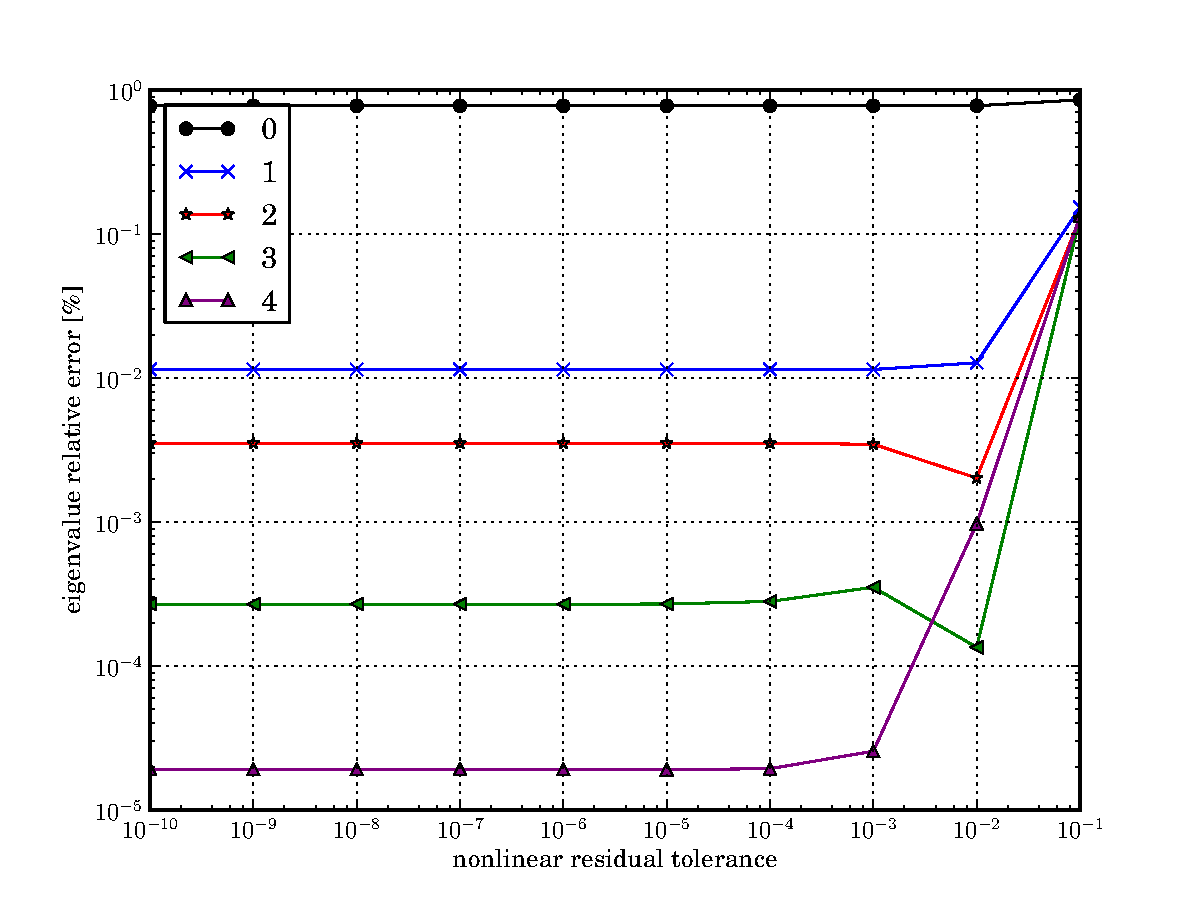
\includegraphics[keepaspectratio, width=1.0\textwidth]
                    {tolerance_study_eigenvalue}
    \caption{Eigenvalue error.}
    \label{fig:tolerance_study_eigenvalue}                   
  \end{subfigure}
  %
  \begin{subfigure}{0.49\textwidth}
    \centering
    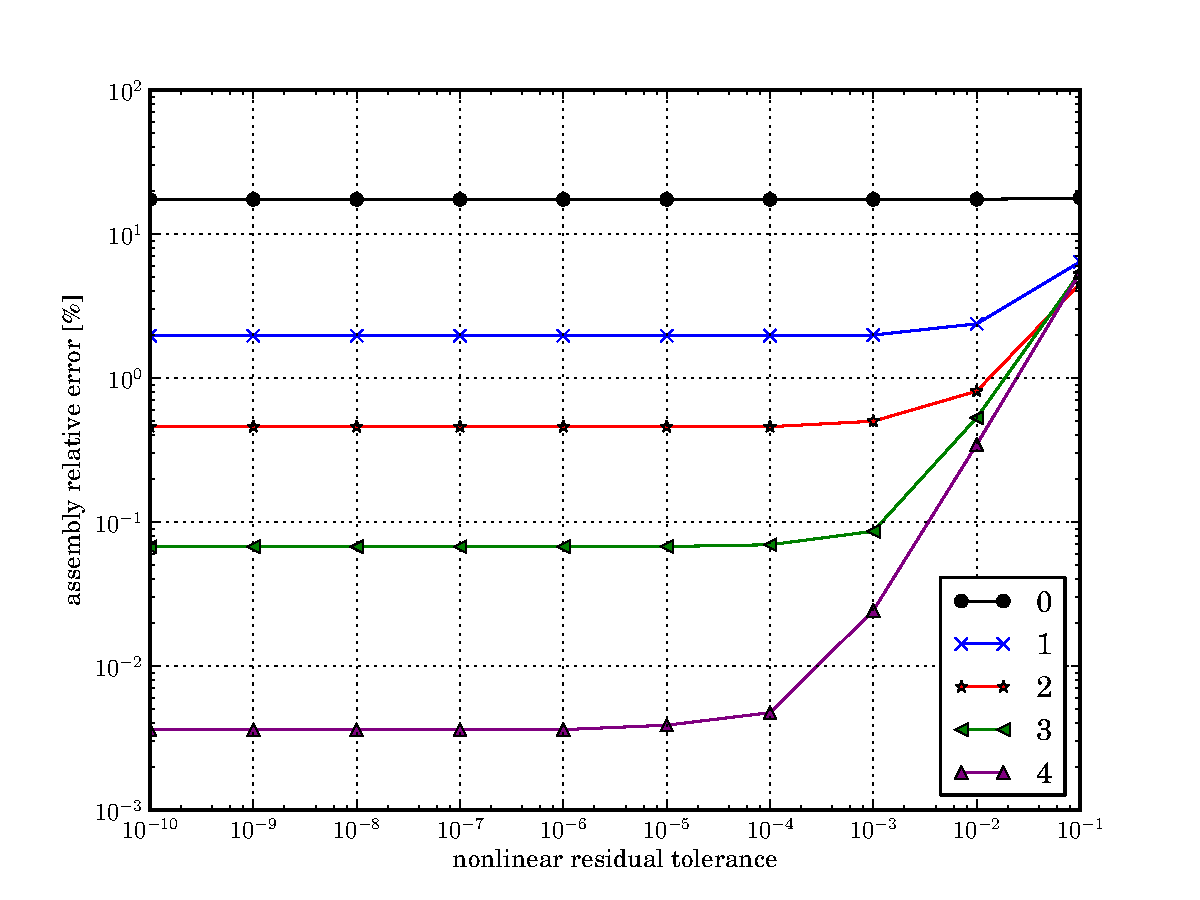
\includegraphics[keepaspectratio, width=1.0\textwidth]
                    {tolerance_study_power}
    \caption{Assembly power error.}
    \label{fig:tolerance_study_power}                 
  \end{subfigure}
  \caption{Absolute relative eigenvalue 
          (\ref{fig:tolerance_study_eigenvalue}) and 
          absolute maximum relative 
          assembly power
           (\ref{fig:tolerance_study_power})
          errors for the 2-D IAEA problem as functions of the
          residual norm tolerance for several spatial orders.}
  \label{fig:tolerance_study}
\end{figure*}

\subsubsection{Orders and Accuracy}
\label{sec:diffusion_order_accuracy}

While a detailed discussion of basis accuracies is outside the 
present scope, it is illustrative to assess convergence 
of the DLP spatial basis applied to the diffusion benchmarks.  
Figure \ref{fig:diffusion_order_study}
 shows the maximum relative error in the assembly 
powers and absolute relative eigenvalue error as functions of spatial order.
For the 
3-D IAEA problem, two approximations were used.  The first is a full 
expansion of order $m$ in both spatial variables, meaning that on a given 
side, the two-dimensional expansion is equivalent to the form 
\begin{equation}
 F(x, y) \approx a + bx + cy + d x^2 + e xy + f y^2 + \ldots \, .
\end{equation}
The second case uses an order reduction scheme that 
limits the sum of the $x$ and $y$ orders \cite{forget2006tdh}.  In this case,
\begin{equation}
 F(x, y) \approx a + bx + cy + d x^2 + f y^2 + \ldots \, ,
\end{equation}
where the cross term $e xy$ has been omitted.  Previous experience 
has demonstrated that these cross terms, particularly at high order, have 
little value, clearly demonstrated in Figure \ref{fig:diffusion_order_study}.

% Say something about the reduction in unknowns, the total node count, 
% etc.

For all the problems, a fourth order expansion yielded assembly 
(or nodal, for the IAEA-3D problem) errors below a tenth of a percent 
and eigenvalue errors on the range of a few pcm.  Consequently, a fourth 
order expansion was selected for use in comparing the solvers in 
subsequent performance analyses.

\begin{figure*}[htbp]
  \centering
  %
  \begin{subfigure}{0.49\textwidth}
    \centering
    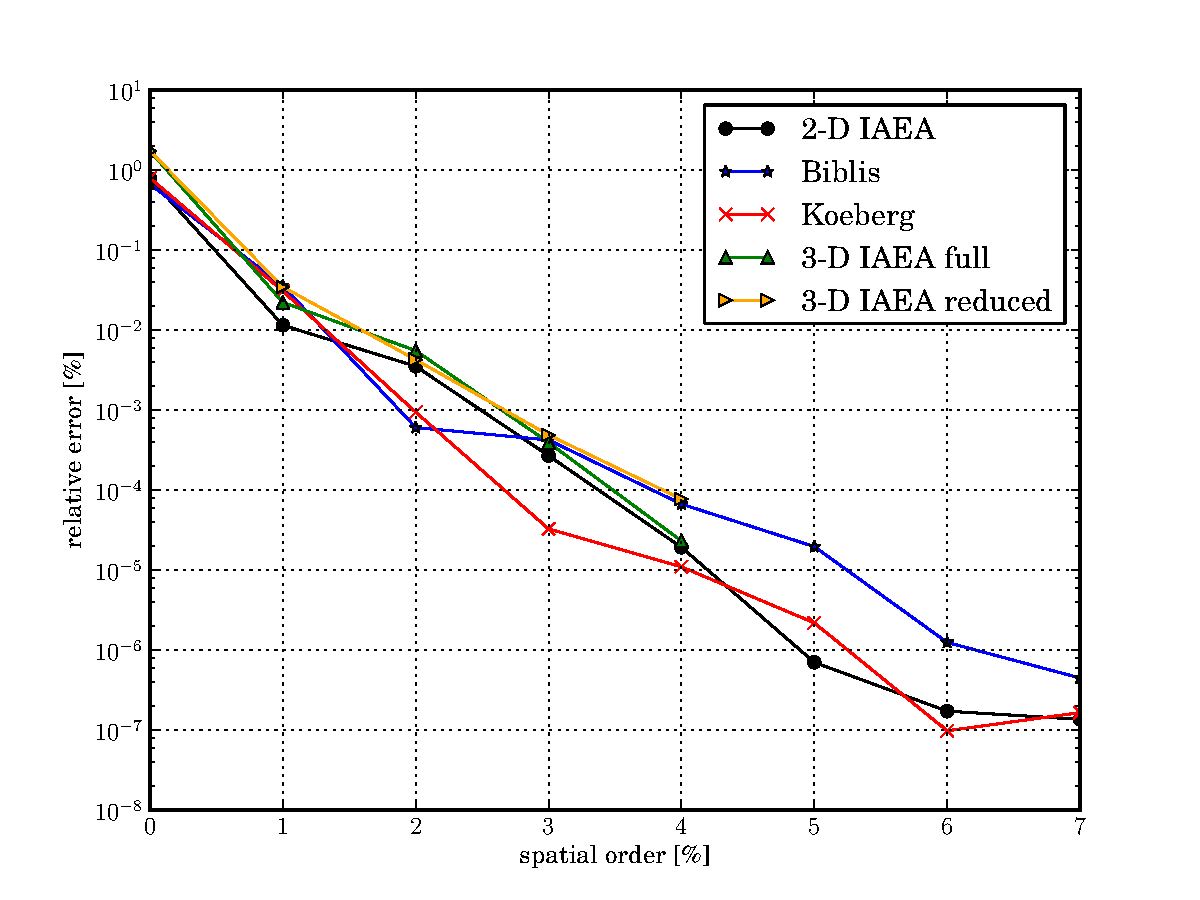
\includegraphics[keepaspectratio, width=1.0\textwidth]
                    {diffusion_order_study_eigenvalue}
    \caption{Eigenvalue error.}
    \label{fig:diffusion_order_study_eigenvalue}                   
  \end{subfigure}
  %
  \begin{subfigure}{0.49\textwidth}
    \centering
    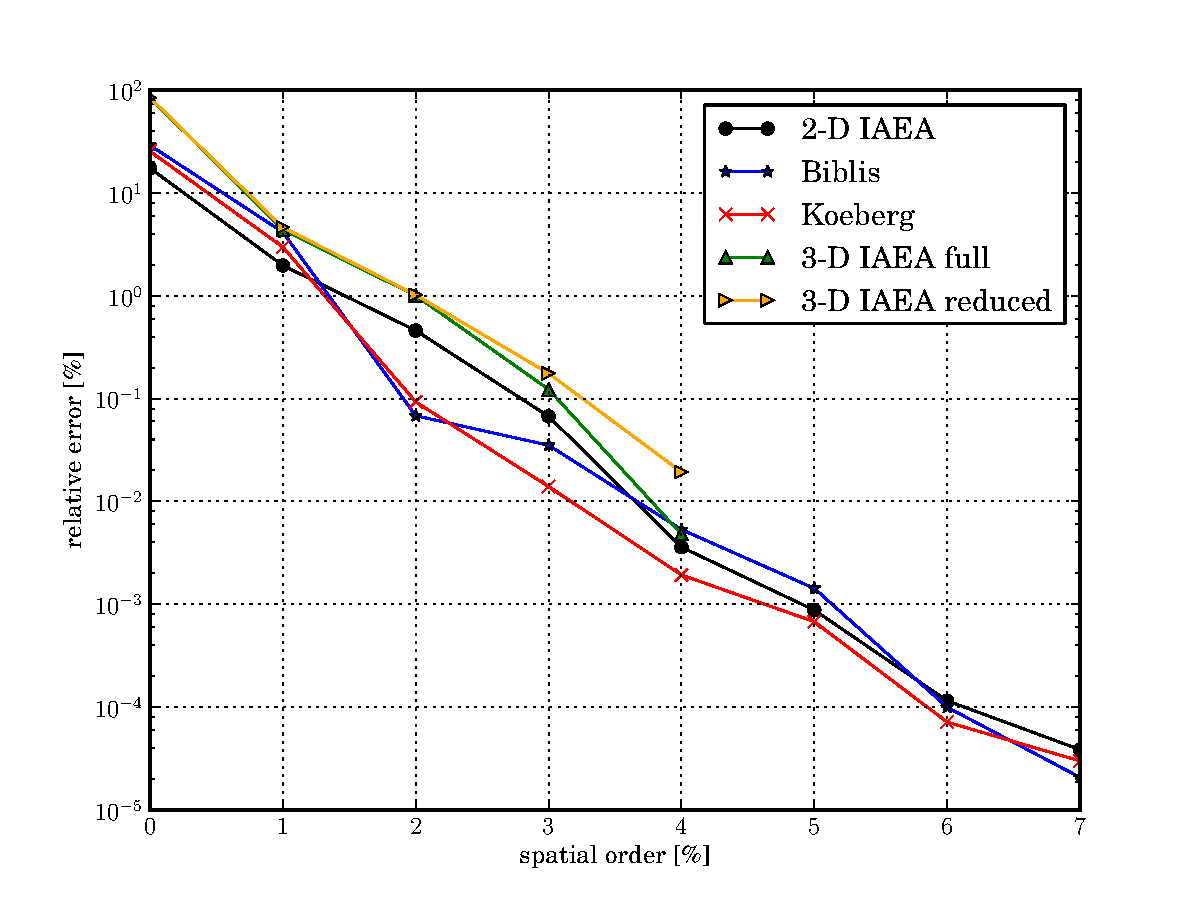
\includegraphics[keepaspectratio, width=1.0\textwidth]
                    {diffusion_order_study_power}
    \caption{Assembly power error.}
    \label{fig:diffusion_order_study_power}                 
  \end{subfigure}
  \caption{Absolute relative eigenvalue 
          (\ref{fig:diffusion_order_study_eigenvalue}) and 
          absolute maximum relative 
          assembly power
           (\ref{fig:diffusion_order_study_power})
          errors as functions of 
          spatial order.}
  \label{fig:diffusion_order_study}
\end{figure*}


\subsubsection{Inner Solver Comparison}

For the Picard solver, several eigenvalue solvers were investigated 
to solve the inner $\lambda$-eigenvalue problem, including the 
power (PI), Krylov-Schur (KS), and explicitly-restarted Arnoldi 
methods (ERAM), which are each
 implemented in SLEPc \cite{slepc}.  Because convergence of the 
outer Picard iteration is  sensitive to the inner convergence, 
the tolerance $\tau_{\lambda}$ of the inner problem was set 
more tightly at $10^{-10}$.  

Table \ref{tbl:diffusion_picard_inner_study} 
provides the number of inner and outer iterations,  total
computational time, and response generation time 
for each method and diffusion problem.
For all problems, 
KS outperforms ERAM by a small margin and PI by a factor of two 
or three.  Initial studies demonstrated that IRAM (not included 
by default with SLEPc) performs at about the same level 
as KS \cite{roberts2012ksi}. Were the tolerance smaller, the improvement 
of KS over PI would 
likely diminish.

For the three 2-D problems, the response time constituted a significant 
portion of the total computational time, ranging from about a third to half
depending on the solver.  For the 3-D IAEA problem, the global solver
was the dominant cost because the diffusion 
problems underlying the response generation are inexpensive compared to 
the much larger global problem.

\begin{table}[ht] 

 \begin{center} 
  \caption{Picard inner solver comparison for diffusion problems.} 
 \label{tbl:diffusion_picard_inner_study} 
 \begin{threeparttable}
 \begin{tabular}{ccccc} 
 \toprule 
  solver & time \tnote{a} & r. time \tnote{b} & inners & outers \\
 \midrule 
              &  \multicolumn{4}{c}{2-D IAEA} \\ 
 \midrule 
           PI &      1.87 &      0.37 &         3416 &            6 \\ 
           KS &      0.69 &      0.41 &           33 &            6 \\ 
         ERAM &      0.77 &      0.40 &           36 &            6 \\ 
 \midrule 
              &  \multicolumn{4}{c}{Biblis} \\ 
 \midrule 
           PI &      2.16 &      0.68 &         3437 &            5 \\ 
           KS &      0.97 &      0.68 &           31 &            5 \\ 
         ERAM &      1.05 &      0.69 &           34 &            5 \\ 
 \midrule 
              &  \multicolumn{4}{c}{Koeberg} \\ 
 \midrule 
           PI &      5.83 &      1.62 &         2012 &            3 \\ 
           KS &      2.38 &      1.66 &           21 &            3 \\ 
         ERAM &      2.63 &      1.67 &           21 &            3 \\ 
 \midrule 
              &  \multicolumn{4}{c}{3-D IAEA} \\ 
 \midrule 
           PI &    910.63 &     18.77 &         4427 &            6 \\ 
           KS &    210.91 &     19.47 &           75 &            6 \\ 
         ERAM &    294.48 &     19.75 &           70 &            6 \\ 
 \bottomrule 
 \end{tabular} 
 

 {\footnotesize
 \begin{tablenotes}
   \item[a] Total time [s]
   \item[a] Response generation time [s]
 \end{tablenotes}
 }
 \end{threeparttable}
 
 
 
 \end{center} 

\end{table} 


\subsubsection{Outer Solver Comparison}

Because KS outperformed the other inner solvers investigated, it was 
selected to study the Picard-based outer iteration schemes.
For this study, Picard iteration, along with the accelerated variant 
based on the {\it regula falsi} method, was compared to Steffensen's 
method and Newton's method.  

\subsubsection{Picard Acceleration}

The four Picard acceleration schemes were applied to the 2-D IAEA 
and Koeberg problems
using a fourth order expansion.  
Figure \ref{fig:diffusion_picard_acceleration}
shows the nonlinear residual as a function of outer iteration for the 
unaccelerated case along with the four accelerated cases. 

Picard iteration alone is a 
rapidly converging process, but acceleration schemes
can further reduce the number of iterations required.
Exponential and inverse-inverse extrapolation provide the 
most robust improvement, although for the Koeberg problem, 
they did not reduce the number of iterations.
The acceleration schemes each critically depend
on the limit $\lambda \to 1$, which is satisfied only if the responses are 
both conservative and computed very accurately.  The 
diffusion equation for each response is small and can be 
solved nearly exactly via LU factorization.  Moreover, the responses 
are conservative 
because a uniform mesh and DLP expansion were used. 
Even so, the linear-inverse and linear-linear suffered from their 
sensitivity to round-off errors, and even though care was taken when 
implementing the coefficients, the convergence tolerances used were 
not tight enough to ensure stability. Because the exponential 
scheme yielded a slightly smaller final residual norm, it was 
included for study with the remaining algorithms.
 
\begin{figure}[ht]
    \centering
    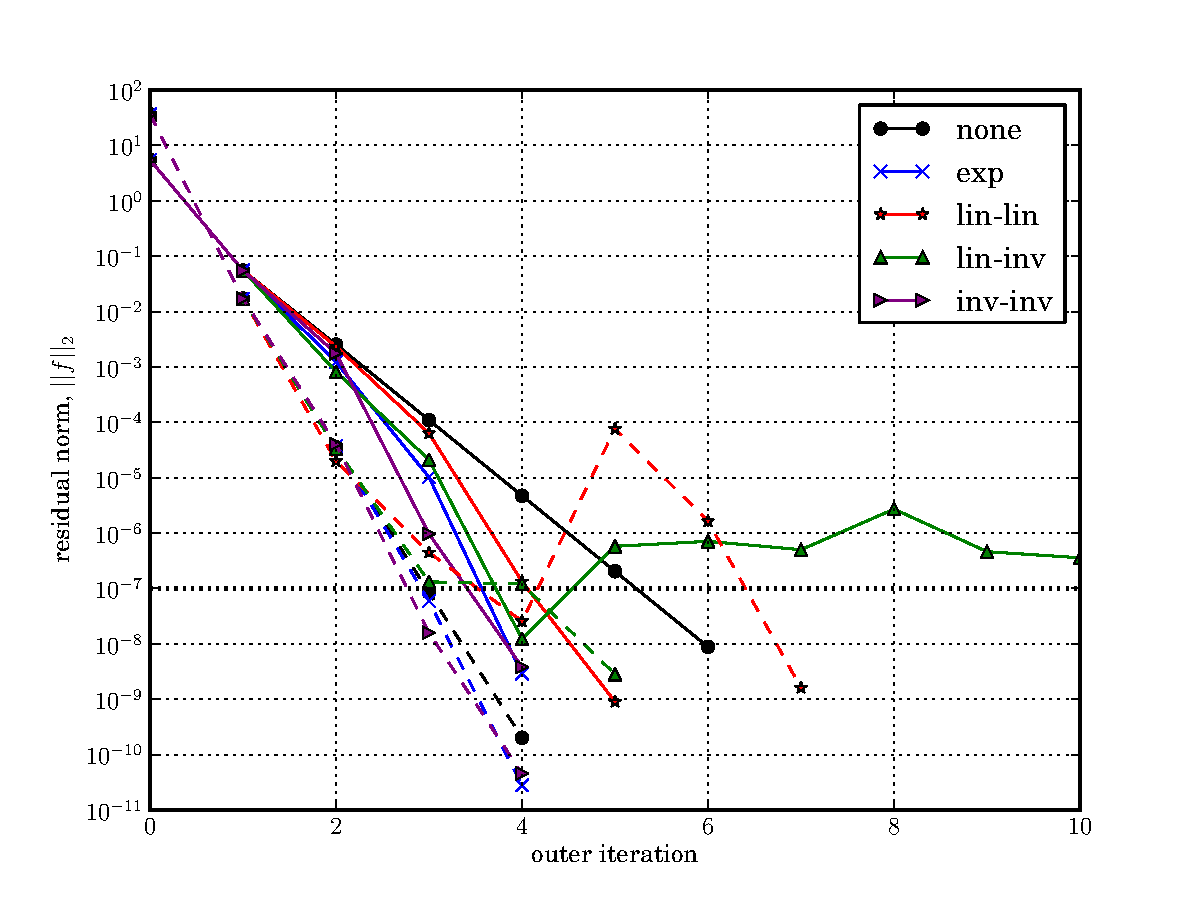
\includegraphics[keepaspectratio, width = 3.5 in]
                    {diffusion_picard_acceleration}
    \caption{Comparison of Picard acceleration schemes for the 
             2-D IAEA problem (solid lines) and Koeberg 
             problem (dashed lines).  }
    \label{fig:diffusion_picard_acceleration}
\end{figure}

\subsubsection{Newton Variants}

For Newton's method, unpreconditioned 
and preconditioned variants using ILU were studied.  The ILU preconditioner
is based on an explicit Jacobian constructed either once, using 
the initial responses, or every iteration, using the updated responses.  
In all cases, the underlying linear solves were performed with GMRES(30),
and the ILU preconditioner was applied with 0 through 2 levels.

Table \ref{tbl:diffusion_newton_pc_study} provides results for the 
2-D IAEA and Koeberg problems with a fourth order spatial 
expansion and $4\times 4$ nodes per assembly, corresponding to
184962 and 369922 unknowns, respectively.
Somewhat larger problems were used to highlight differences between
the preconditioners because the preconditioners offered no benefit 
for the single node case.

For both problems, ILU(0) preconditioning offered the best performance
with respect to time, although higher preconditioner levels 
led to lower numbers of inner iterations.
Failure to update the preconditioner had no discernible effect 
on the iteration count and yielded lower computational times than when 
the preconditioner was updated at every iteration.  This can be explained 
by noting that a majority of the Jacobian is relatively insensitive 
to small changes in $k$.  Given the initial guess for $k$ 
(unity in these cases)
is expected to be pretty close to the final answer, the original Jacobian
should be nearly equal to its final value.

\begin{table}[ht] 
 
 \begin{center} 
  \caption{Newton solver ILU preconditioner comparison for diffusion 
          problems.} 
 \label{tbl:diffusion_newton_pc_study}
 \begin{threeparttable}

 \begin{tabular}{ccccc} 
 \toprule 
  preconditioner & time\tnote{a} & r. time\tnote{b} & inners & outers \\
 \midrule 
 &  \multicolumn{4}{c}{2-D IAEA} \\ 
 \midrule 
          none &     12.62 &      0.46 &          477 &            4 \\ 
  no update ILU(0) &     10.43 &      0.46 &          144 &            4 \\ 
  no update ILU(1) &     11.68 &      0.46 &          118 &            4 \\ 
  no update ILU(2) &     12.37 &      0.46 &           86 &            4 \\ 
        ILU(0) &     10.69 &      0.46 &          144 &            4 \\ 
        ILU(1) &     14.07 &      0.45 &          118 &            4 \\ 
        ILU(2) &     17.12 &      0.45 &           86 &            4 \\ 
 \midrule 
 &  \multicolumn{4}{c}{Koeberg} \\ 
 \midrule 
          none &     45.82 &      3.29 &          403 &            4 \\ 
  no update ILU(0) &     43.18 &      3.34 &          157 &            4 \\ 
  no update ILU(1) &     52.18 &      3.35 &          136 &            4 \\ 
  no update ILU(2) &     58.26 &      3.35 &           91 &            4 \\ 
        ILU(0) &     45.61 &      3.35 &          157 &            4 \\ 
        ILU(1) &     67.44 &      3.38 &          136 &            4 \\ 
        ILU(2) &     89.90 &      3.35 &           91 &            4 \\ 
 \bottomrule 
 \end{tabular} 
 

 {\footnotesize
 \begin{tablenotes}
   \item[a] Total time [s]
   \item[b] Response generation time [s]
 \end{tablenotes}
 }
 \end{threeparttable}
 
 
 \end{center} 

\end{table} 

\subsubsection{Comparing Picard, Steffensen, and Newton}
\label{sec:global_solver_diffusion}

Several metrics can be used to compared the outer solvers. Ultimately, 
wall clock time is most important in practice.  However, the number of 
iterations 
of each method, both outer and inner, is also indicative of the 
algorithm performance, independent of any particular implementation.
These data are provided in Table \ref{tbl:diffusion_outer_study} 
for each of the benchmarks. A fourth
order spatial expansion  was used for all problems, with order reduction 
applied to the 3-D IAEA problem.  For the 2-D problems, a $4\times 4$ 
node-per-assembly model was used, while for the 3-D IAEA problem,  
a single node was used, corresponding to 184962 unknowns for the 
2-D IAEA and Biblis problems, 369922 for the Koeberg problem, 
and 988382 for the 3-D IAEA problem.

\begin{table*}[ht] 

 \begin{center} 
 
 \caption{Outer solver comparison for diffusion problems.} 
 \label{tbl:diffusion_outer_study} 
 
 \begin{threeparttable}
 \begin{tabular}{cccccc} 
 \toprule 
  solver & time\tnote{f}  & r. time\tnote{g} & inners & outers & $k$-evals. \\
 \midrule 
 &  \multicolumn{5}{c}{2-D IAEA} \\ 
 \midrule 
    P\tnote{a}        &     10.26 &      0.32 &           76 &            5 &            6 \\ 
    P+exp\tnote{b} &      9.09 &      0.27 &           65 &            4 &            5 \\ 
    S\tnote{c} &     11.20 &      0.39 &           80 &            3 &            7 \\ 
  N+$\delta k$\tnote{d} &     10.35 &      0.44 &          144 &            4 &            8 \\ 
  N+$\Delta k$\tnote{e} &     10.22 &      0.28 &          146 &            4 &            5 \\ 
 \midrule 
 &  \multicolumn{5}{c}{Koeberg} \\ 
 \midrule 
        P &      9.26 &      0.56 &           64 &            4 &            5 \\ 
    P+exp &      9.06 &      0.56 &           62 &            4 &            5 \\ 
    S &      9.36 &      0.56 &           64 &            2 &            5 \\ 
  N+$\delta k$ &     10.89 &      0.92 &          140 &            4 &            8 \\ 
  N+$\Delta k$ &     10.49 &      0.57 &          140 &            4 &            5 \\ 
 \midrule 
 &  \multicolumn{5}{c}{Biblis} \\ 
 \midrule 
    P &     25.65 &      1.61 &           54 &            3 &            4 \\ 
    P+exp &     25.76 &      1.62 &           54 &            3 &            4 \\ 
    S &     29.61 &      2.02 &           60 &            2 &            5 \\ 
  N+$\delta k$ &     43.10 &      3.26 &          157 &            4 &            8 \\ 
  N+$\Delta k$ &     42.07 &      2.05 &          157 &            4 &            5 \\ 
 \midrule 
 &  \multicolumn{5}{c}{3-D IAEA} \\ 
 \midrule 
        P &    213.51 &     17.93 &           75 &            6 &            7 \\ 
    P+exp &    167.93 &     12.79 &           62 &            4 &            5 \\ 
    S &    214.07 &     17.98 &           75 &            3 &            7 \\ 
  N+$\delta k$ &    269.36 &     20.93 &          129 &            4 &            8 \\ 
  N+$\Delta k$ &    261.27 &     13.02 &          129 &            4 &            5 \\ 
 \bottomrule 
 \end{tabular} 

 {\footnotesize
 \begin{tablenotes}
   \item[a] Picard 
   \item[b] Picard with exponential extrapolation
   \item[c] Steffensen
   \item[d] Newton with fine $k$ difference
   \item[e] Newton with coarse $k$ difference
   \item[f] Total time [s]
   \item[g] Response generation time [s]
 \end{tablenotes}
 }
 \end{threeparttable}
 
 \end{center} 
 
\end{table*} 

%  \footnote{fine finite difference for $k$}
%  \footnote{coarse finite difference for $k$}

The tested solvers include Picard (P) with and without exponential 
extrapolation (exp), Steffensen's method (S), and Newton's method (N).
For Newton's method, two schemes were examined.  The first is the same 
as used for testing the preconditioning and is based on a Jacobian with 
$k$-derivatives computed using a finite difference 
with a $\Delta k = 10^{-8}$.
The second scheme uses the two most recent $k$ values
for computing $\Delta k$, resulting in a larger $\Delta k$ and, therefore, 
a less accurate finite difference.  However, the accuracy of the finite 
difference did not affect the convergence, 
and for all four problems,
the coarse difference yielded the same number of outer iterations as the 
fine difference while reducing the number of $k$ evaluations by nearly half.

Steffensen's method provided the fastest convergence with respect to 
outer iterations, but it requires two $k$ evaluations per outer iteration.
Picard with exponential extrapolation yielded the lowest computational 
time and the fewest $k$ evaluations.  While Newton's method with a 
coarse $\Delta k$ is competitive with respect to $k$ evaluations, the 
overhead of solving the linear systems is higher than the cost of the 
$\lambda$-eigenvalue problem in the Picard iteration.

% FIGURE

\subsubsection{Comments}

Based on these diffusion analyses, Picard iteration with
KS for the inners and exponential extrapolation for accelerating 
the outers represents an ideal ERMM solver.  The Newton methods yield 
perform 
nearly as well with respect to $k$ evaluations, but the cost of 
applying the method is higher per iteration than the Picard variants,
implying further work on preconditioning the inner solves is warranted.

\subsection{2-D C5G7}

The 2-D C5G7 transport benchmark is a small quarter core 
model consisting of two UO$_2$ assemblies and two MOX
assemblies, all surrounded by an assembly-width reflector.  The model 
is based on 7 group data and homogenization of the fuel and cladding.
 
\subsubsection{Orders and Accuracy}
 
To assess the accuracy of the response schemes available for transport 
problems, the C5G7 benchmark was solved using a variety of 
angular bases. Because a uniform spatial mesh was 
not used, the DLP spatial expansion converged more slowly for 
the C5G7 problem than for the 
uniformly-meshed diffusion problems.  For all cases, 
the response transport calculations were converged to 
a relative residual norm of $10^{-8}$, and the outer calculation was 
converged to a nonlinear residual norm of $10^{-7}$.

Table \ref{tbl:c5g7_order_convergence} shows the convergence of 
the eigenvalue and pin power errors as a function of space-angle 
order.  By third order, the conservative basis yields
very limited improvement, most likely due to the DLP 
spatial basis used.  A nonuniform mesh yields a nonconservative
DLP expansion that is inaccurate at low orders compared to a
conservative expansion.
Table \ref{tbl:c5g7_order_convergence} shows that both the
DLP and Chebyshev bases yield
maximum relative pin power errors of slightly more than 2\%.
These results are in contrast to results reported in 
Ref. \cite{roberts2014psb}, 
which used a full order spatial basis to eliminate spatial errors and
showed that a conservative Chebyshev basis significantly outperforms a
DLP basis.
Consequently, the present results indicate that
spatial expansion errors are dominant by second or third order,
and, therefore, a full 
implementation and systematic study of new spatial bases 
is warranted.

\begin{table*}[ht] 
 
\begin{center} 

 \caption{2-D C5G7 order convergence.  All errors in \%, with 
          reference MCNP results from the original documentation.} 
 \label{tbl:c5g7_order_convergence} 

  \begin{threeparttable}
 \begin{tabular}{ccrrrrrr} 
 \toprule 
 basis & order & $e_k$\tnote{a}   & $\max |e_i|$\tnote{b}  & $ \frac{\max |e_i|}{p^{\text{ref}}_i} $  
   & $\frac{\sum_i |e_i|}{ N}$   &  $\frac{\sqrt{\sum_{i} e_{i}^2}}{N}$   
     & $ \frac{\sum_i |e_i|p^{\text{ref}}_i}{N} \bar{p}^{\text{ref}}$    \\
 \midrule 
 DLP-$\psi$  &    0  &     1.00   &    33.32   &   109.45   &     9.41   &     0.36   &    10.97   \\
 DLP-$\psi$  &    1  &     0.72   &    38.17   &    18.49   &     2.65   &     0.12   &     3.06   \\
 DLP-$\psi$  &    2  &     0.13   &     4.36   &     7.49   &     0.98   &     0.04   &     1.36   \\
 DLP-$\psi$  &    3  &     0.01   &     2.20   &     5.81   &     0.37   &     0.02   &     0.42   \\
 \midrule 
 Chebyshev-$\psi$  &    0  &     2.61   &    40.43   &   107.58   &     9.46   &     0.37   &    10.86   \\
 Chebyshev-$\psi$  &    1  &     0.07   &    19.93   &    11.38   &     0.99   &     0.05   &     1.22   \\
 Chebyshev-$\psi$  &    2  &     0.04   &     2.73   &     6.28   &     0.39   &     0.02   &     0.40   \\
 Chebyshev-$\psi$  &    3  &     0.04   &     2.27   &     6.00   &     0.35   &     0.02   &     0.38   \\
 \midrule 
 {\tt Detran}\tnote{c} & n/a  &     0.01   &     0.91   &     0.94   &     0.17   &     0.01   &     0.22   \\

% detran as reference
% DLP-$\psi$ &    0  &     1.00   &    33.35   &   108.87   &     9.49   &     0.36   &    11.11   \\
% DLP-$\psi$  &    1  &     0.72   &    37.78   &    18.52   &     2.63   &     0.12   &     3.07   \\
% DLP-$\psi$  &    2  &     0.13   &     4.67   &     7.74   &     0.92   &     0.04   &     1.25   \\
% DLP-$\psi$  &    3  &     0.01   &     2.35   &     6.24   &     0.35   &     0.02   &     0.37   \\
%  \midrule 
% Chebyshev-$\psi$ &    0  &     2.61   &    40.73   &   107.01   &     9.57   &     0.37   &    11.03   \\
% Chebyshev-$\psi$ &    1  &     0.07   &    19.54   &    11.09   &     1.01   &     0.06   &     1.26   \\
% Chebyshev-$\psi$ &    2  &     0.04   &     2.95   &     6.70   &     0.39   &     0.02   &     0.37   \\
% Chebyshev-$\psi$ &    3  &     0.04   &     2.42   &     6.43   &     0.35   &     0.02   &     0.35   \\
 \bottomrule 
 \end{tabular}  
 {\footnotesize
 \begin{tablenotes}
   \item[a] $e_k = |k-k^{\text{ref}}|/k^{\text{ref}}$  
   \item[b] $e_i = p_i - p^{\text{ref}}_i$, for $i$th pin
   \item[c] based on {\tt Detran} solution of the C5G7 problem with the same
            discretization and quadrature and, thus, represents the lower error 
            bound for {\tt Serment} 
 \end{tablenotes}
 }
 
 \end{threeparttable}
 
 \end{center} 

\end{table*} 

\subsubsection{Solver Comparison}

The same global solvers used in 
Section \ref{sec:global_solver_diffusion} were also applied 
to the 2-D C5G7 problem.  In this case, 64 processes were used 
for response generation, while a
single process was used for the outer ($\lambda$-eigenvalue) problem.

Table \ref{tbl:c5g7_outer_study} provides the wall time,
as well as the total and response time summed over all 
processes.  In addition, the number of inner iterations,
outer iterations, and $k$ evaluations are included. Newton's method with the 
coarse $k$ derivative yielded the best performance, with a wall 
time of $1.09\cdot 10^3$ seconds, total 
time of $6.97\cdot 10^4$ seconds (summed over 
all processes), and a solver (excluding response generation) time of 
$34$ seconds. Use of 
the fine $k$ derivative required more outer iterations and, consequently, 
significantly more time.  Steffensen's method required the 
fewest outer iterations but at the 
cost of more $k$ evaluations.  Standard Picard iteration 
readily converged, but extrapolation
failed miserably.  However, this failure is {\it completely expected}: 
the spatial basis is not conservative, so $\lambda$ does not 
tend toward unity, and, hence, extrapolation does not apply.  This 
highlights significant value in selecting a conservative basis, 
because the extrapolated Picard iteration was the best performing 
method for the diffusion problems.

\begin{table*}[ht] 
 \begin{center} 
 \caption{Outer solver comparison for 2-D C5G7 problem with first order expansions.
          Picard with exponential extrapolation fails due to the nonconservative spatial 
          basis, \ie $\lambda \ne 1$.} 
 \label{tbl:c5g7_outer_study} 
  \begin{threeparttable}
 \begin{tabular}{ccccccc} 
 \toprule 
  solver & w. time\tnote{f} & time\tnote{g} & r. time\tnote{h} & inners & outers & $k$-evals. \\
  \midrule
    P\tnote{a}            &  $1.67\cdot 10^3$ &  $1.07\cdot 10^5$ &  $1.07\cdot 10^5$ &           16 &            6 &            7 \\ 
    P+exp\tnote{b}        &  $6.26\cdot 10^3$ &  $4.00\cdot 10^5$ &  $4.00\cdot 10^5$ &           36 &           21 &           21 \\ 
    S\tnote{c}            &  $1.73\cdot 10^3$ &  $1.11\cdot 10^5$ &  $1.11\cdot 10^5$ &           16 &            3 &            7 \\ 
    N+$\delta k$\tnote{d}            &  $4.60\cdot 10^3$ &  $2.94\cdot 10^5$ &  $2.94\cdot 10^5$ &           76 &            8 &           16 \\ 
    N+$\Delta k$\tnote{e} &  $1.09\cdot 10^3$ &  $6.97\cdot 10^4$ &  $6.96\cdot 10^4$ &           33 &            4 &            5 \\ 
 \bottomrule 
 \end{tabular} 
 
 {\footnotesize
 \begin{tablenotes}
   \item[a] Picard 
   \item[b] Picard with exponential extrapolation
   \item[c] Steffensen
   \item[d] Newton with fine $k$ difference
   \item[e] Newton with coarse $k$ difference
   \item[f] Wall time [s]
   \item[g] Total time summed over all processes [s]
   \item[h] Total response generation time summed over all processes [s]
 \end{tablenotes}
 }
 
 \end{threeparttable}
 
 \end{center} 

\end{table*} 

\subsection{3-D Takeda}

The 3-D Takeda benchmark is a simple benchmark, but it
allows for in-depth examination of the convergence properties of 
the basis sets.  The model consists of three homogeneous regions using 
a two group approximation in energy.  For this study, the the ``rods in''
configuration was used.

\subsubsection{Order Convergence}

Figures \ref{fig:takeda_order_study_eigenvalue_error} and
\ref{fig:takeda_order_study_nodal_power_error} provide the absolute 
relative error in the eigenvalue and the maximum 
absolute relative error in the nodal powers as a function of angular 
order for several spatial orders.  Order reduction was used in 
both space and angle.  Very little improvement was observed
with increasing angular order for a spatial order of zero.  
For higher spatial orders, an increasing angular order 
yielded a monotonically decreasing error for both $k$ and the nodal 
powers.  The conservative basis outperformed the DLP variants, yielding
nearly sub-1\% nodal errors for a third order angular expansion and 
spatial orders greater than one.  DLP-$J$ yielded slightly 
better nodal powers than DLP-$\psi$ at higher orders but higher 
$k$ errors for all orders. 

For all angular bases, a significant trend observed was the markedly
diminishing returns for spatial orders above 
two.  In other words, the most consistent improvement observed,
irrespective of angular order and basis, was obtained by shifting 
from first to second order in space.  This trend is reasonable because 
the nodes are homogeneous, and boundary quantities should, therefore, 
be relatively smooth functions of space.

\begin{figure*}[htbp]
  \centering
  %
  \begin{subfigure}{0.49\textwidth}
    \centering
    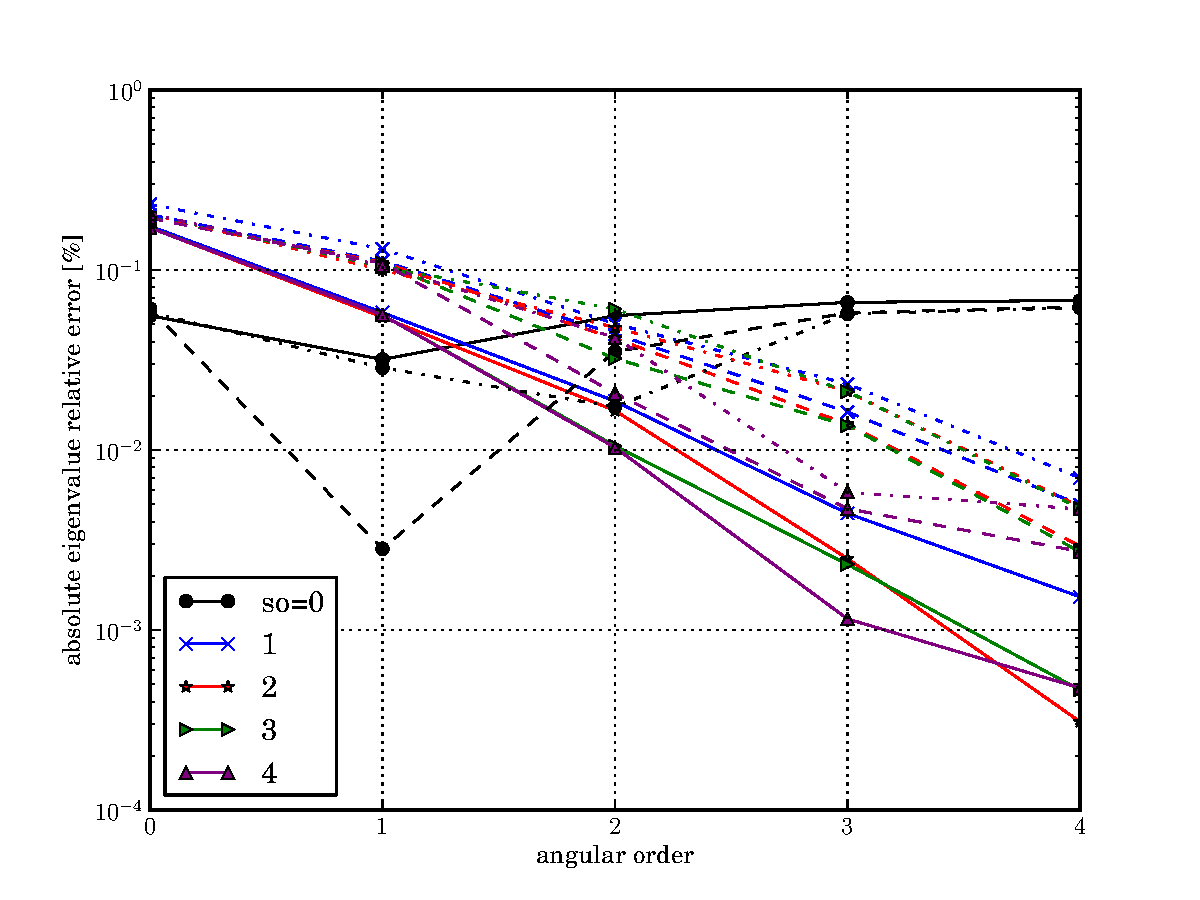
\includegraphics[keepaspectratio, width=1.0\textwidth]
                    {takeda_order_study_eigenvalue_error}
    \caption{Eigenvalue error.}
    \label{fig:takeda_order_study_eigenvalue_error}                   
  \end{subfigure}
  %
  \begin{subfigure}{0.49\textwidth}
    \centering
    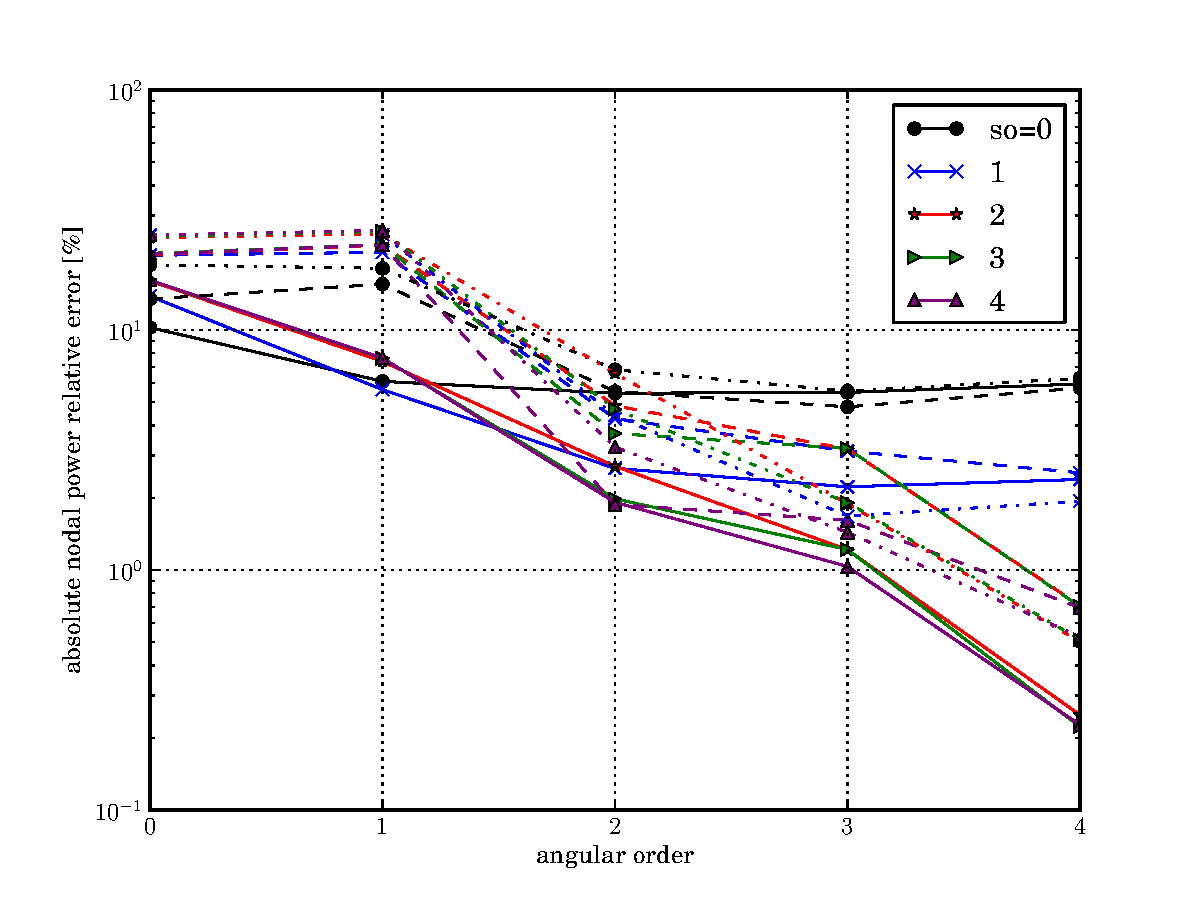
\includegraphics[keepaspectratio, width=1.0\textwidth]
                    {takeda_order_study_nodal_power_error}
    \caption{Nodal power error.}
    \label{fig:takeda_order_study_nodal_power_error}                 
  \end{subfigure}
  \caption{Takeda problem absolute relative 
           eigenvalue (\ref{fig:takeda_order_study_eigenvalue_error})
           and nodal power (\ref{fig:takeda_order_study_nodal_power_error})
           errors as 
           a function of angular order for several spatial orders.  
           The solid lines indicate the conservative basis, while the 
           dashed and dashed-dot lines indicate the DLP basis used to 
           expand the angular flux $\psi$ and current $J$, respectively.}  
  \label{fig:core_benchmark_plot}
\end{figure*}

\subsubsection{Solver Comparison}

The same solvers used for the diffusion  
and 2-D C5G7 problems were applied to the Takeda problem. A second 
order spatial expansion with a third order angular expansion in the 
azimuth and polar variables was used.  Order reduction was applied to 
the spatial and angular terms.  The problem was run with 64 processes, with 
one process for the global problem.  Table \ref{tbl:takeda_outer_study} 
provides the wall time, total time summed over all processors, and the 
total response function time summed over all processors.  

Similar to the diffusion results, the extrapolated Picard iteration 
proved to be the most efficient of the solvers studied.  
Newton's method with the coarse $k$ finite difference yielded just as 
few $k$ evaluations but with a slightly higher overall cost.

\begin{table*}[ht] 
 \begin{center} 
 \caption{Outer solver comparison for 3-D Takeda problem with second order 
          spatial expansion and third order polar and azimuthal angle 
          expansions.} 
 \label{tbl:takeda_outer_study} 
  \begin{threeparttable}
 \begin{tabular}{ccccccc} 
 \toprule 
  solver & w. time\tnote{f} & time\tnote{g} & r. time\tnote{h} & inners & outers & $k$-evals. \\
  \midrule
    P\tnote{a}            &  $9.76\cdot 10^2$ &  $6.25\cdot 10^4$ &  $5.91\cdot 10^4$ &           56 &           13 &           14 \\ 
    P+exp\tnote{b}       &  $3.51\cdot 10^2$ &  $2.24\cdot 10^4$ &  $2.12\cdot 10^4$ &           23 &        4 &   5  \\ 
    S\tnote{c}            &  $1.05\cdot 10^3$ &  $6.72\cdot 10^4$ &  $6.36\cdot 10^4$ &           58 &            7 &           15 \\ 
    N+$\delta k$\tnote{d}&  $7.30\cdot 10^2$ &  $4.67\cdot 10^4$ &  $4.26\cdot 10^4$ &           57 &            5 &           10 \\ 
    N+$\Delta k$\tnote{e}&  $3.87\cdot 10^2$ &  $2.48\cdot 10^4$ &  $2.14\cdot 10^4$ &           44 &          4 &           5  \\ 
 \bottomrule 
 \end{tabular} 
 
 
 {\footnotesize
 \begin{tablenotes}
   \item[a] Picard 
   \item[b] Picard with exponential extrapolation
   \item[c] Steffensen
   \item[d] Newton with fine $k$ difference
   \item[e] Newton with coarse $k$ difference
   \item[f] Wall time [s]
   \item[g] Total time summed over all processes [s]
   \item[h] Total response generation time summed over all processes [s]
 \end{tablenotes}
 }
 
 \end{threeparttable}
 
 \end{center} 
\end{table*} 

\section{Conclusion}
\label{sec:conclusion}

Based on the results for both the diffusion and transport problems, Picard 
iteration with exponential extrapolation appears to be the most
efficient method studied, yielding minimum numbers of $k$ evaluations 
while providing the lowest global solver overhead.  However,  
extrapolation is based on $\lambda$ converging to unity, and because this 
is not always guaranteed, Newton's method with the coarse finite difference 
provides a more consistently robust solver, with nearly as 
few $k$ evaluations and only relatively small overhead due to the 
inner linear solves.

Further work on preconditioners for Newton's method 
will likely reduce the corresponding (global) computation time 
to levels similar to extrapolated Picard iteration.  
Even so, the efficacy and 
simplicity of Picard iteration suggests that care should be taken to 
select a conservative basis leading to $\lambda = 1$ upon convergence.

Ultimately, the present work supports broader efforts to use 
ERMM for production level analyses, but significant challenges remain,
dominated by the vast number of responses required for realistic 
modeling.  Solvers were developed that reduce the number of $k$ evaluations 
required and minimize time spent generating  
responses, while related recent work successfully developed diffusion-based 
transport preconditioners that significantly reduce the time of 
individual response calculations \cite{roberts2014dpm}.  Because 
responses are independent, parallel computation will be a natural
component of 
any future ERMM implementation.  Scoping studies have demonstrated 
nearly ideal scaling of {\tt Serment} on a small research 
cluster \cite{roberts2014arm}, and ongoing work aims to test {\tt Serment} on 
leadership-class machines.

\section*{Acknowledgements}

The work of the first author was supported in part by a
Department of Energy Nuclear Energy University Programs Graduate Fellowship.
Additionally, the authors wish to thank one of the reviewers
for comments that helped clarify aspects of the early response 
matrix literature.

\end{document}
